\documentclass[notitlepage]{article}

\usepackage[margin=2cm]{geometry}

\usepackage{amsmath}
\usepackage{amsfonts}
%\usepackage{braket}
\usepackage{tabularx}
\usepackage{amsthm}
\usepackage[braket, qm]{qcircuit}
%\usepackage[bookmarks = true, pdfpagemode = None, pdfstartview = FitH, colorlinks = true, urlcolor = blue]{hyperref}
\usepackage{listings}
\lstset{
	basicstyle=\small\ttfamily,
	columns=flexible,
	breaklines=true
}
\usepackage{caption}
\usepackage{subcaption}
\usepackage{graphicx}
\usepackage{algorithm}
\usepackage{placeins}
%\usepackage{algorithmic}
\usepackage[noend]{algpseudocode}
\makeatletter
% Reinsert missing \algbackskip
\def\algbackskip{\hskip-\ALG@thistlm}
\makeatother
\renewcommand{\arraystretch}{1.5}

\theoremstyle{definition}
\newtheorem{definition}{Definition}[section]

\theoremstyle{problem}
\newtheorem{problem}{Problem}[section]

\theoremstyle{lemma}
\newtheorem{lemma}{Lemma}[section]

\usepackage{pdfpages}
%\usepackage{epspdfconversion}
\usepackage{xcolor,colortbl}
\usepackage{wrapfig}
\usepackage{multirow}

\title{Efficient Algorithms for Multi-Qubit Circuit Optimization}
\title{An Efficient Quantum Compiler with Near-Optimal $T$ Count}
\author{Luke Heyfron and Earl T. Campbell}
\date{October 2017}

\begin{document}
	\maketitle
	\begin{abstract}
		% THIS PAPER
In order to perform quantum algorithms on a real quantum computer, one must first decompose the algorithm into machine-level instructions compatible with the architecture of the quantum computer, a process known as quantum compiling.
In principle, there are many different quantum circuit decompositions for the same algorithm and due to the expense of running a quantum computer, it is desirable to compile into circuits that minimize space-time cost metrics. A popular measure of cost is the $T$ count, which emerges from the prevalent Clifford + $T$ magic states model of fault-tolerant quantum computing and closely approximates the full space-time cost for high-threshold quantum error correction codes such as the toric code.
The problem of optimizing the $T$ count of a quantum circuit, or gate synthesis, is a relatively young area of research but exciting progress has been made, especially for the single qubit case which is essentially a solved problem. However, multi-qubit gate synthesis is believed to be a hard problem with optimal algorithms requiring classical runtime exponential in the number of qubits, $n$. Conversely, the best known polynomial-time algorithms either solve special cases that restrict us to a non-universal gate set or make no promises with regards to global optimality. In this paper, we present a quantum compiler for multi-qubit Clifford + $T$ quantum circuits that is both fast with runtime polynomial in $n$ and near-optimal in the sense that the output quantum circuit has $T$ count with worst case scaling of $\mathcal{O}(n^2)$, which is the same scaling as that of the optimal inefficient algorithm and smaller than the best previous heuristic by a factor $n$. We have implemented several variants of this protocol in C++ and benchmark tested them on random circuits, from which we determine that Third Order Duplicate and Destroy (TODD) yields the lowest $T$ counts on average. Also, we ran our compiler on a library of circuits that implement quantum algorithms in order to compare with previous works and found that in each case our protocol generates circuits with lower $T$ counts than the best known previous algorithm, providing solid evidence that our protocol is the forerunner amongst Clifford + $T$ quantum compilers.
		
		% QEC POSTER
		%Quantum computers are expensive to run in practice, motivating us to minimize the amount of time and space resources consumed by executing quantum algorithms. Quantum circuits allow us to decompose complex quantum algorithms into elementary quantum gates. However, the cost of each gate is not necessarily uniform - rather we must take into consideration the quantum error correction (QEC) code used to protect our quantum memory from noise. High-threshold codes such as the 2D surface code \cite{29_Dennis_2002} only natively support a limited set of operations, requiring expensive extra steps to realise universal quantum computation. The magic states model \cite{32_Bravyi_2005} is one of the leading proposals for fault-tolerant quantum computations and assumes that so called Clifford operations are free and implies that the cost of a circuit is proportional to the number of uses of the $T$ gate, or the $T$-count of a circuit. We consider the gate synthesis problem of finding circuit decompositions with minimal T count that implement a given $n$ qubit unitary generated by the Clifford + T gate set. There are no known optimal solvers for this problem that are computationally efficient in the number of qubits. Moreover, the problem is believed to be hard. Therefore, it is desirable to develop efficient algorithms that yield near-optimal solutions. To this end, we present an efficient near-optimal T gate optimization algorithm that yields lower T counts than the best known previous algorithms, which we have implemented in C++ along with competing algorithms.
		
		% QEC POSTER APPLICATION
		%In order to realise practical quantum computation, it is important to consider the resource cost associated with implementing quantum circuits. The T gate requires several hundred times more elementary operations than Clifford group operators to implement fault-tolerantly for certain high-threshold quantum error correction codes such as the toric code. Therefore, effective methods for minimizing the number of T gates in a given quantum circuit are instrumental in reducing the overall cost of quantum computation. Finding the minimum number of T gates required to implement an $n$-qubit circuit generated by CNOT and T has been shown to be equivalent to minimum distance decoding of the punctured Reed-Muller code of length $n$ and order $n-4$, which is believed to be a hard problem. In this poster, we present two computationally efficient heuristics for estimating the minimal number of T gates required for multi-qubit circuits generated by CNOT and T gates. Both algorithms output circuits with T counts that have asymptotic scaling $\mathcal{O}(n^2)$, which is the same scaling as the upper bound for the inefficient optimal decoder. The algorithms can be adapted for circuits over the universal $\{\text{H}, \text{CNOT}, \text{T}\}$ gate set by allowing for ancilla preparation and classical feedforward and have been used to estimate the T count for known practical quantum circuits.
		
		% FIRST YEAR REPORT
		%In order to realise practical quantum computation, it is important to consider the resource cost associated with implementing quantum circuits. The T gate, also called the $\pi/8$ phase gate, requires several hundred times more elementary operations than Clifford group operators to implement fault-tolerantly for certain high-threshold quantum error correction codes such as the surface code. Therefore, effective methods for minimizing the number of T gates in a given quantum circuit are instrumental in reducing the overall cost of quantum computation. Finding the minimum number of T gates required to implement an $n$-qubit circuit generated by CNOT and T has been shown to be equivalent to minimum distance decoding of the punctured Reed-Muller code of length $n$ and order $n-4$, which is believed to be a hard problem. In this report, we present two computationally efficient heuristics for estimating the	minimal number of T gates required for multi-qubit circuits generated by CNOT and T gates. One of the algorithms, based on Lempel's factoring algorithm, outputs circuits with T counts that scale asymptotically as $\mathcal{O}(n^2)$, which is the same scaling as the upper bound for the inefficient optimal decoder and improves upon the worst-case scaling of $\mathcal{O}(n^3)$ for a naive fast decoder. Numerics obtained for the other algorithm, which we call \emph{LempelX}, suggest that it also has $\mathcal{O}(n^2)$ scaling. The algorithms can be adapted for circuits over the universal $\{H,CNOT,T\}$ gate set by allowing for ancilla preparation and classical feedforward, and we used LempelX to estimate the T count for known practical quantum circuits.
		
		% LIT. REVIEW
		% In order to realise practical quantum computation, it is important to consider the resource cost associated with implementing a particular sequence of quantum gates. The T-gate is known to require many more steps to implement fault-tolerantly than Clifford gates for certain high-threshold quantum error correction codes such as the toric code. Therefore, it is desirable to reduce the number of `expensive' T-gates used to implement a given quantum circuit. We review the best known protocols for finding the minimal number of T-gates required to construct a given quantum circuit (the T-count) and protocols for synthesising instances of quantum circuits that use minimal T-gates. We look in particular at an algorithm solving the multi-qubit exact gate synthesis problem for circuits composed from elementary Clifford gates and the T-gate; as well as a more specialised and faster algorithm for circuits composed of CNOT and T-gates based on Reed-Muller minimum distance decoding.
	\end{abstract}
	
	\section{Introduction}
		% Motivation:
		% 	- Use an example of optimal run time on a known circuit to motivate development of efficient heuristics.
		%	- (T gates are expensive)
		%	- Problem definition: exact multi-qubit non-unitary Clifford + T synthesis problem
		%	- Motivate problem: exact optimal single qubit synthesis essentially solved; multi-qubit believed to be hard; by relaxing problem to allow for non-unitary processes such as ancillas and measurements we have developed an efficient Clifford + T near optimal gate synthesis protocol by borrowing from techniques for symmetric tensor contracting on GF(2).
		%	- Paper overview: Section 1 intoduction and motivation; section 2, 3 description of the high and low levels respectively of the T gate optimization protocol main result of this paper. Section 4 discuss results for T counts numerical resultant from this algorithm and compared to others. Section 5 Discuessions and conclusions for future work.
		\iffalse
		T gates are expensive toric code transversal gates high threshold Clifford operations.		
		exact optimal single qubit synthesis essentially solved; multi-qubit believed to be hard; by relaxing problem to allow for non-unitary processes such as ancillas and measurements we have developed an efficient Clifford + T near optimal gate synthesis protocol by borrowing from techniques for symmetric tensor contracting on GF(2).
		exact multi-qubit non-unitary Clifford + T synthesis problem given an n qubit input circuit U that can be synthesized exactly using gate from Clifford + T gate set, find a circuit U' on n+h qubits that implements U on the first n qubits and the final h qubits are not entangled with the first n using minimal number of T gates.
		We have developed an efficient T-gate optimization protocol that finds nearly optimal solutions to the above problem.
		An overview of the paper is as follows. Section 1 introduction and motivation; section 2, 3 description of the high and low levels respectively of the T gate optimization protocol main result of this paper. Section 4 discuss results for T counts numerical resultant from this algorithm and compared to others. Section 5 Discussions and conclusions for future work.
		\fi
		
		Compiling is the conversion of an algorithm into a series of hardware level commands or elementary gates.   A more optimal compiler can implement the same algorithm using fewer hardware level instructions, reducing runtime and other resources.  Quantum compiling or gate-synthesis is the analogous task for a quantum computer and is especially important given the current expense of quantum hardware.  At the very dawn of quantum computing as a field, Solovay and Kitaev proposed a general purpose compiler that was compatible with any universal set of elementary gates~\cite{kitaev02,dawson05,fowler11}.  Unfortunately, it was far from optimal, generating circuits using many more gates than are necessary.   
		
		After a long lull, recent years have brought a series of significant improvements in compiling methods.  This new generation of compilers exploit the specific structure of the Clifford+$T$ gate set, reducing quantum circuit depths by several orders of magnitude and also often improving the classical compile time~\cite{kliuchnikov13,selinger13,gosset14,RS14}.   Focus on this gate set is warranted since it naturally appears as the set of logical gates in almost every fault-tolerant computing architecture~\cite{ReviewPaper}.  Furthermore, proposed fault-tolerant devices often use techniques, such as magic state distillation~\cite{BraKit05},  where the cost per $T$ gate is several hundreds of Clifford gates~\cite{RHG01a,Fowler12,gorman17}.  This suggests $T$ count as the key metric of compiler performance.
		
		Significant progress has been made on synthesis of single-qubit unitaries from Clifford+$T$ gates.  For purely unitary synthesis, the problem is essentially solved since we have a compiler that is optimal and efficient~\cite{kliuchnikov13,RS14}, with a command line implementation freely available~\cite{gridsynth}.  Yet further improvements are possible beyond unitary circuits, by making use of ancilla qubits and measurements~\cite{paetznick14,bocharov15,bocharov15b} or adding an element of randomness to compiling~\cite{campbell17shorter,hastings2016mixing}.  Whereas, the multi-qubit problem is much more challenging.  An algorithm for multi-qubit  unitary synthesis over the Clifford+$T$ gate set is known that is provably optimal in terms of the $T$ count but the compile runtime is exponential in the number of qubits~\cite{gosset14}.  More recently, a highly efficient compiler has been developed that is effective at reducing not only the $T$ count but also the CNOT and continuous phase gate counts, but it makes no promises regarding global optimality~\cite{2067}. Instead, we seek a compiler that runs efficiently with circuit size and yields $T$ counts as close to the global minimum as possible, with some prior attempts at this goal~\cite{amy2013meet}. 
		
		A useful strategy for multi-qubit synthesis is to take an initial Clifford+$T$ circuit and split it into partitions containing Hadamards and partitions containing CNOT, $S$ and $T$ gates.  One can then attempt to reduce the number of $T$ gates within just the latter partitions.  Amy and Mosca recently shows that this restricted synthesis problem is formally equivalent to error decoding on a class of Reed-Muller codes~\cite{amy16}, which is in turn equivalent to finding the symmetric tensor rank of a 3-tensor~\cite{seroussi80}.  Unfortunately, even this easier sub-problem is  NP-complete to solve optimally.  Nevertheless, this problem does seem more amenable to efficient solvers that offer reductions in $T$ count.  Amy and Mosca argued that an $n$-qubit subcircuit (containing CNOT, $S$ and $T$ gates) has an optimal decomposition into $n^2/2+O(n)$ $T$ gates.  At the time,  known efficient compilers could only promise an output circuit with no more than $O(n^3) $ $T$ gates.  Later, Campbell and Howard~\cite{campbell17b} sketched a compiler that is efficient and promises an output circuit with at most $n^2/2+O(n)$ $T$ gates.  This shows efficient compilers can in this sense be ``near-optimal" with respect to worst case scaling.   On the mathematical level, Campbell and Howard exploited a previously known efficient and optimal solver for a related 2-tensor problem~\cite{lempel75} but suitably modified so that it nearly-optimally solves the required 3-tensor problem.
		
		This paper develops several different compilers that are efficient and near-optimal in the above sense. We provide the first implementations of such compilers and provide performance comparison against: a family of random circuits; and a library of circuits taken from actual quantum algorithms.  For random circuits, we find the actual performance follows the worst-case scaling for different compilers.  We observe  $O(n^2)$ scaling for all variants of our compiling approach compared with $O(n^3)$ scaling for compilers based on earlier work.   For actual quantum algorithms, the full Clifford+$T$ gate set is needed and so our compiler also makes use of a gadgetisation tricks to eliminate Hadamards and convert the problem to synthesis over just the CNOT, $S$ and $T$ gate set.  Quantum algorithms are highly structured and far from random, so the number of $T$ gates can not be meaningfully compared with the worst case $n$ scaling.  Instead, we benchmark against the best previously known results.  We  find our compilers gave significant reductions in $T$ count for almost every circuit tested and never gave worse $T$ counts.
		
		All of the near-optimal compilers described in this paper look for inspiration in algorithms for the related 2-tensor problem, which we call the Lempel's algorithm.  We give specific details for a compiler here called TOOL (Target Optimal by Order Lowering) that comes in two different flavours (with and without feedback).  The TOOL compilers can be considered concrete versions of the approach outlined by Campbell and Howard~\cite{campbell17b}.  Also proposed in this paper is the TODD (Third Order Duplicate and Destroy) compiler, which is again inspired by Lempel but in a more direct and elegant way than TOOL.  In benchmarking, we find that TODD often achieved even lower $T$ count than TOOL.  
		
	\FloatBarrier
	
	\section{Preliminaries}	
	% Clifford heirarchy, D_3
	The Pauli group on $n$ qubits $\mathcal{P}^n$ is the set of all $n$-fold tensor products of the single qubit Pauli operators $\{X, Y, Z, \mathbb{I}\}$ with allowed coefficients $\in \{\pm1,\pm i\}$.
	The Clifford group on $n$ qubits $\mathcal{C}^n$ is the normalizer of $\mathcal{P}^n$.
	The $k$\textsuperscript{th} level of the \emph{Clifford hierarchy} $\mathcal{C}_k^n$ is defined as follows,
	\begin{equation}
	\label{e_heir}
	\mathcal{C}_k^n = \{U \mid U\mathcal{P}^n U^\dagger = \mathcal{C}_{k-1}^n\},
	\end{equation}
	with recursion terminated by $\mathcal{C}^n_1 = \mathcal{P}^n$.
	We define $\mathcal{D}_k^n$ to be the diagonal elements of $\mathcal{C}_k^n$. We will omit the superscript $n$ when the number of qubits is obvious from context.
	% Gate sets used: Clifford + T, CNOT + T
	%We define the Clifford + $T$ gate set $\mathcal{G}_1 = \{\mathrm{Clifford}, T\}$, where Clifford is any generating set for the Clifford group on $n$ qubits such as $\{CNOT,H,S\}$.
	We define Clifford to be any generating set for the Clifford group on $n$ qubits such as $\{CNOT,H,S\}$.
	We define the CNOT + $T$ gate set to be $\{\mathrm{CNOT}, S, T\}$, where we include the phase gate $S=T^2$ as a separate gate due to the magic states cost model for gate synthesis \cite{BraKit05}.
	A quantum circuit decomposition for a unitary $U$ is denoted $\mathcal{U}$; conversely we say $\mathcal{U}$ implements $U$. Similarly, a circuit $\mathcal{E}$ implements non-unitary channel $\rho \rightarrow \varepsilon(\rho)$. We refer to a circuit $\mathcal{U}$ that implements a $U\in \mathcal{D}_3$ as a \emph{diagonal} CNOT + $T$ \emph{circuit}. We define $\circ$ to be an operator that composes two circuits together in left-to-right time order.
	
	% Most general circuit optimization problem
	
		
	\section{Workflow Overview}
		\label{sec_methods}
		\label{ssec_workflow}

%\begin{lstlisting}
% 0/in) The input
%	- A circuit decomposition \mathcal{U} \in <G_1>
%	- A netlist i.e. a list of quantum gate each with the qubits to which they are applied.
%	- Allowed gates in this group in our implementation are {X,Y,Z,S(^dagger),T,T(^dagger),CZ,CS(^dagger) and CCZ}
%	- Non-unitary implementations of gates lower down Clifford hierarchy such as generalized Toffoli gate as described in appendix B

% 1) Remove external Hadamards

% 2) Clifford + T to CNOT + T mapping
%	- Replace H gates with gadget in figure \ref{fig_hadamards}
%	- Pauli X operator commutes through the CNOT+T partitions (reference to new figure)

% 3) Diagonalize CNOT + T circuit
%	- Action of an arbitrary circuit in G2 on computational basis states is fully described by phase polynomial + l.b.f, however l.b.f's can be implemennted using only CNOTs which is Clifford so it is convenient to focus on only diagonal CNOT + T gates, allowing us to ignore the l.b.f.
%	- Consequently, we decompose the CNOT + T circuit into a diagonal CNOT + T circuit and a CNOT only circuit that implements the l.b.f

% 4) Determine the `phase function decompositions' of diagonal CNOT + T circuit
%	- Weighted polynomial
%	- Phase polynomial
%	- Signature tensor
%	- Gate synthesis matrix
%	- Reference to mappings figure
%	- Original WP/PP must be stored in order to later apply the Clifford correction that restores U_{POST} to U_{PRE} (due to losing information that contains Clifford behaviour in the WP->ST, PP->GSM mappings)

% 5) Find T-optimal phase function decomposition A

% 6) Map A back to diagonal CNOT + T circuit
%	- Determine Clifford correction from stored WP/PP

% 7/out) The output
%\end{lstlisting}

\begin{figure}[h!]		
	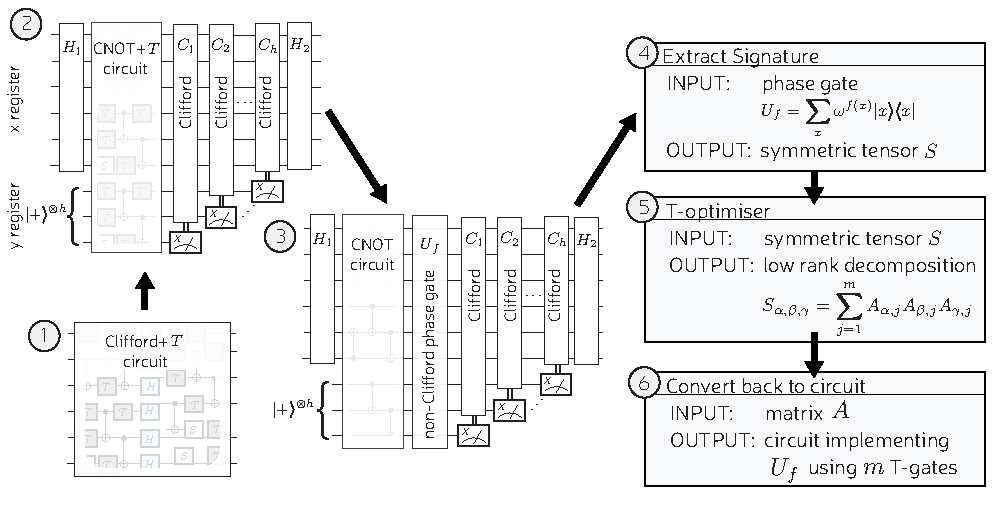
\includegraphics{Overview4b}
	\caption{The high level workflow of the T gate optimization protocol is shown. A Clifford + T circuit is converted to the CNOT+T gate set by introducing ancillas and performing classically controlled Clifford gates. A non-Clifford phase gate is extracted, which maps to a signature tensor upon which the core optimization algorithm is performed. The optimized symmetric tensor decomposition is then converted back into a circuit of the form in panel 2) yielding an implementation of the original Clifford + T circuit with reduced T count. }
	\label{fig_overview}
\end{figure}

% in)
We now describe the high level work-flow of our $T$ gate optimization protocol.
The input and output of the protocol are quantum circuit decompositions that are defined in terms of two distinct qubit registers, labelled x and y. The x (y) register is composed of $n$ ($h$) qubits and spans the Hilbert space $\mathcal{H}_{\text{x}}$ ($\mathcal{H}_{\text{y}}$). The input circuit, $\mathcal{U}_{\text{in}} \in \langle \mathrm{Clifford}, T \rangle$, implements a unitary $U \in \mathcal{C}_3^n$. The output, $\mathcal{E}_{\text{out}}  \in \langle \mathrm{Clifford}, T, M, \ket{+}, \mathrm{feedforward} \rangle $, is a circuit also composed of Clifford and $T$ gates but additionally allows: the preparation of $\ket{+}$ states; measurement in the Pauli-X basis, $M$, and classical feedforward. $\mathcal{E}_{\text{out}}$ implements the non-unitary quantum operator $\varepsilon_{\text{out}}:\mathcal{H}_{\text{x}} \mapsto \mathcal{H}_{\text{x}}\otimes \mathcal{H}_{\text{y}}$ given by
\begin{equation}
\label{e_out_1}
\varepsilon_{\text{out}}(\rho_{\text{x}}) = \varepsilon_{\text{post}}(U_{\text{out}}(\rho_{\text{x}}\otimes\rho_{\text{y}})U_{\text{out}}^\dagger),
\end{equation}
where $\rho_{\text{x}}$ is the density matrix for an arbitrary input pure state on $\mathcal{H}_\text{x}$, and $\rho_{\text{y}}=(\ket{+}\bra{+})^{\otimes h}$ is a density matrix on  $\mathcal{H}_\text{y}$. $U_{\text{out}}\in \mathcal{C}_3$ is the unitary portion of $\mathcal{E}_{\text{out}}$, and $\varepsilon_{\text{post}}$ is a quantum channel that is associated with the sequence of Pauli-$X$ measurements and subsequent classically controlled Clifford gates, $C_1^{m_1},C_2^{m_2},\dots,C_h^{m_h}$, seen in figure \ref{fig_overview}. $\mathcal{E}_{\text{out}}$ is synthesized such that, once we trace out the y register from the result of $\varepsilon_{\text{out}}$ acting on $\rho_{\text{x}}$, we recover the input unitary,
\begin{equation}
\label{e_out_2}
\mathrm{Tr}_{\text{y}}(\varepsilon_{\text{out}}(\rho_{\text{x}})) = U\rho_{\text{x}}U^\dagger.
\end{equation}

\iffalse\begin{figure}[h]
	\[
	\Qcircuit @C=1em @R=1em {
		\lstick{\ket{\psi}} & \gate{H} &  \rstick{H\ket{\psi}}\qw & &\push{\rule{2em}{0em}=\rule{2em}{0em}} & 
		\lstick{\ket{\psi}} & \ctrl{1} & \qw & \qswap & \qw & \gate{X} & \rstick{H\ket{\psi}}\qw & &\push{\rule{2em}{0em}=\rule{2em}{0em}} &
		\lstick{\ket{\psi}} & \gate{S} & \ctrl{1} & \qw & \targ & \ctrl{1} & \gate{X} & \rstick{H\ket{\psi}}\qw \\
		& & & & &
		\lstick{\ket{+}} &  \ctrl{-1} & \qw & \qswap \qwx & \qw & \meter \cwx & \dstick{X} & & &
		\lstick{\ket{+}} &  \gate{S} & \targ & \gate{S^\dagger} & \ctrl{-1} & \targ & \meter \cwx & \dstick{X}
	}
	\]
	\caption{Internal Hadamards are removed by replacing each one according to this circuit identity. The Hadamards on the left-hand circuit are now external and act on an ancilla, therefore they no longer obstruct the \emph{T-optimiser} algorithms. The classically controlled Pauli-$X$ correction of each Hadamard gadget must be conjugated through to the end of the circuit in order to maximize the extent of the CNOT+$T$ sub-circuit of figure \ref{fig_overview}.2. Because circuits generated by CNOT+$T$ form a group within the third level of the Clifford heirarchy, the conjugation of a Pauli operator through this circuit leads to classically controlled Clifford operators $C_1, C_2, \dots, C_h$ in figure \ref{fig_overview}.2 and \ref{fig_overview}.3.}
	\label{fig_hadamards}
\end{figure}\fi

\begin{figure}[h!]
	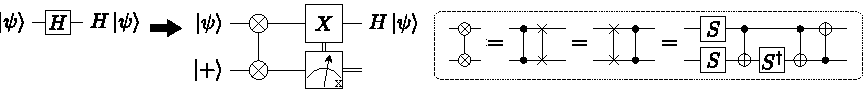
\includegraphics[width=\linewidth]{phaseswap}
	\caption{Hadamard gates are replaced by Hadamard-gadgets according to the rewrite rule on the LHS. On the RHS, we define notation for the phase-swap gate and provide an example decomposition into the CNOT + $T$ gate set.}
	\label{fig_hadamards}
\end{figure}

% 1,2)
We will describe the process of our protocol in 6 steps. First, we emphasize that \emph{T-Optimiser} makes use of a framework valid only for CNOT + $T$ circuits, which makes Hadamard gates as obstacles. We overcome this in steps 1 and 2 using methods based on reference \cite{1_Montanaro_2017}. First, we remove external Hadamards
%(those that appear at the beginning or end of the circuit)
from $\mathcal{U}_{\text{in}}$ and place them into circuits $H_1$ and $H_2$ for those that appear at the beginning and end of the circuit, respectively. Then in step 2, each of the $h$ internal Hadamard gates is replaced by a \emph{Hadamard-gadget} as shown in figure \ref{fig_hadamards}. A Hadamard-gadget consists of a CNOT + $T$ block followed by a Pauli-$X$ gate conditioned on the outcome of measuring a \emph{Hadamard-ancilla} (a qubit in the y register initialized in the $\ket{+}$ state) in the Pauli-$X$ basis. Each internal Hadamard that appears in $\mathcal{U}_{\text{in}}$ invokes a new Hadamard-ancilla, so the size of the y register is $h$. After making the initial Hadamard to Hadamard-gadget substitution, we commute the classically controlled Pauli-$X$ gates to the end of the circuit, starting with the right-most and iteratively working our way left  (see figure \ref{f_comm}). The end result is a circuit composed of a single CNOT+$T$ block on $n+h$ qubits, followed by a sequence of classically controlled Clifford operators conditioned on Pauli-$X$ measurements. The latter sequence of non-unitary gates constitutes the circuit $\mathcal{E}_{\text{post}}$. This method of circumventing Hadamards is preferred over that of forming Hadamard-bounded partitions as in previous works \cite{6_Amy_2013} because it allows us to convert most of the input circuit into the optimization-compatible gate set, which we find leads to better performance of the \emph{T-Optimize} subroutine.

\begin{figure}
	\begin{equation}
	\begin{array}[t]{c @{{}={}} c @{{}={}} c}
	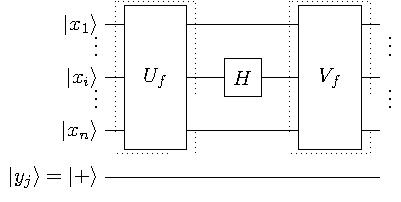
\includegraphics[width=0.3\linewidth]{cc1} & 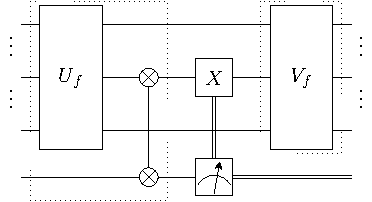
\includegraphics[width=0.3\linewidth]{cc2b} & 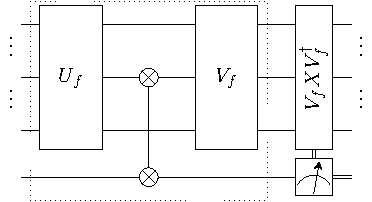
\includegraphics[width=0.3\linewidth]{cc3b}
	\end{array}
	\end{equation}
	\caption{Example showing a Hadamard gate swapped for a Hadamard-gadget where the classically controlled Pauli-$X$ gate is commuted through to the end. The CNOT + $T$ -only region increases as shown by the dotted lines. Note that $V_f X V_f^\dagger \in \mathcal{C}_2$ as per equation \ref{e_heir}, so has a $T$-count of $0$.}
	\label{f_comm}
\end{figure}

% 1)
\iffalse In fact, we do not need to convert every Hadamard gate into `Hadamard gadgets'. As in previous works \cite{1_Montanaro_2017}, we make a distinction between \emph{internal} and \emph{external} Hadamards, where we define the former to be any Hadamard gate this is located such that there is at least one non-commuting gate acting on the same qubit line immediately before and after it. We define an external Hadamard as any Hadamard that is not an internal Hadamard. In step 1, external Hadamards are detached from the input circuit before gadgetization in step 2 as shown in panels 2 and 3 of figure \ref{fig_overview}. This saves space-like resources as each additional Hadamard gadget requires one additional ancilla qubit, resulting in the number of Hadamard gadgets $h=h_{\text{total}}-h_{\text{external}}$, where $h_{\text{total}}$ and $h_{\text{external}}$ are the total number of Hadamard gates and the number of external Hadamards in $\mathcal{U}_{\text{in}}$, respectively.\fi

% 3)
Once the internal Hadamards are removed, we are left with a CNOT + $T$ circuit 
%$\mathcal{U}_{CNOT+T}$
that implements unitary $U_{CNOT+T}$, whose action on the computational basis is fully described by two mathematical objects: a \emph{phase function}, $f: \mathbb{Z}_2^n \mapsto \mathbb{Z}_8$, and an invertible matrix $E \in \mathbb{Z}_2^{(n,n)}$, such that
\begin{equation}
U_{CNOT+T}\ket{\mathbf{x}} = \omega^{f(\mathbf{x})}\ket{E\mathbf{x}}
% \\&= \omega^{f(\mathbf{x})}\left(\ket{\lambda_1(\mathbf{x})}\otimes\ket{\lambda_2(\mathbf{x})}\otimes\dots\otimes\ket{\lambda_n(\mathbf{x})}\right),
\end{equation}
where $\omega = e^{i\frac{\pi}{4}}$. It can be shown that a circuit $\mathcal{U}_E$ that implements the transform $U_E\ket{\mathbf{x}}=\ket{E\mathbf{x}}$ needs only the CNOT gate. It is convenient to strip away this Clifford behaviour and focus on \emph{diagonal} CNOT + $T$ circuits that require only the phase function for a full description of the unitary.
Hence in step 3, we decompose $\mathcal{U}_{CNOT+T}$ into two partitions: $\mathcal{U}_E$ and $\mathcal{U}_f$, the latter being a diagonal CNOT + $T$ circuit that implements $U_f$, whose action is given by
\begin{equation}
\label{e_U_f_wo}
U_f\ket{\mathbf{x}} = \omega^{f(\mathbf{x})}\ket{\mathbf{x}}.
\end{equation}

\begin{wrapfigure}{r}{0.4\linewidth}
	\centering
	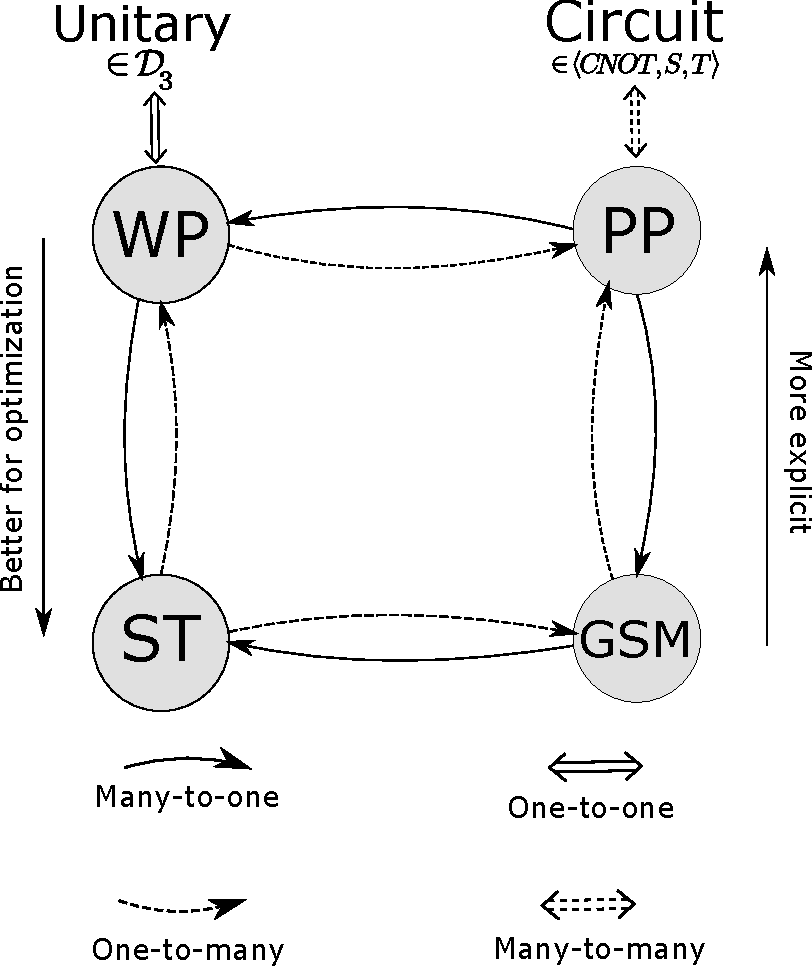
\includegraphics[width=1\linewidth]{maprep}
	\caption{Phase function representations}
	\label{fig_maprep}
\end{wrapfigure}

% 4)
We make use of four different \emph{phase function representations}: \emph{phase polynomials} (PP), \emph{weighted polynomials} (WP), \emph{gate synthesis matrices} (GSM) and \emph{signature tensors} (ST), which are mappable to one another, as well as to and from the unitary and circuit descriptions as shown in figure \ref{fig_maprep}. The mathematical definition of each representation and some of their mappings will be covered in section \ref{ssec_diag}. For now, we will highlight relative merits of each.
Phase polynomials map to quantum circuits, where the number of $T$ gates required is a known function of the PP coefficients.
%They also retain the Clifford behaviour of the input unitary, so are more explicit than GSMs.
There exist many different PPs for the same unitary that in general have different $T$ counts, wherein lies the $T$ optimization problem. On the other hand, weighted polynomials have a one-to-one correspondence with the unitary it implements, a property we exploit to check that our optimization methods leave the input unitary invariant. The signature tensor is a streamlined version of the WP that ignores the Clifford behaviour irrelevant for $T$ optimization. Finally, gate synthesis matrices are streamlined versions of PPs, similarly with the Clifford behaviour ignored. In step 4, we extract the phase function representations of $\mathcal{U}_f$ and store them in memory.



% 5)
The key subroutine of the algorithm, \emph{T-optimiser}, is performed in step 5. It takes as input the signature tensor, $S$, of $U_f$ and outputs a gate synthesis matrix, $A$, with $m$ columns such that $S^{(A)} = S^{(U_f)}$. For $T$-optimal circuits, the output of \emph{T-optimiser} has minimal $m$, but finding optimal GSMs is believed to be a hard problem as we will expand upon in section \ref{s_topt}. We have implemented a number of heuristic versions of \emph{T-optimiser} that yield GSMs with near-minimal $m$, which are described in detail in section \ref{s_topt}.



% 6)
In the final step, we map the output GSM of $\emph{T-optimiser}$ to a diagonal CNOT + $T$ circuit, $\mathcal{U}_{f^\prime}$, that comprises $m$ instances of the $T$ gate using lemma \ref{l_gsm2circ}. The circuit $\mathcal{U}_{f^\prime}$ implements a unitary $U_{f^\prime}=U_fU_{\text{Clifford}}$, where $U_{\text{Clifford}}$ is a diagonal Clifford factor. The input WP stored since step 4 contains sufficient information to generate a circuit for $U_{\text{Clifford}}^\dagger$ (see appendix \ref{ap_Cliff}), hence we recover the original unitary, $U_f=U_{f^\prime} U_{\text{Clifford}}^\dagger$. The final part of step 6 constitutes replacing $\mathcal{U}_f$ with $(\mathcal{U}^\dagger_{\text{Clifford}}\circ\mathcal{U}_{f^\prime})$. At this stage, the protocol terminates returning the final output, $\mathcal{E}_{\text{out}} = (H_1\circ \mathcal{U}_E \circ \mathcal{U}^\dagger_{\text{Clifford}}\circ\mathcal{U}_{f^\prime} \circ \mathcal{E}_{\text{post}}\circ H_2)$, which has near-minimal $T$ count.

% Need to note somewhere that we also do a post-processing stage to cancel adjacent pairs of U U^dagger gates.

\iffalse  It takes as input the signature tensor, $S$, of $\mathcal{U}_{f}$ and outputs a gate synthesis matrix, $A$, with near-minimal column number such that the ST of $A$ is $S$. The number of columns of $A$ is equal the number of $T$ gates required to implement $A$ as a quantum circuit, so \emph{T-optimiser} ideally outputs a gate synthesis matrix with minimal column number. It is believed that finding optimal solutions for this problem is NP-hard \cite{3_Amy_2016}, so we must use efficient heuristics that yield near-minimal column number.

The output $A$ matrix is mapped to a circuit of the same form as $U_f$, with which the original $U_f$ circuit is replaced. The result is an output circuit that implements the full Clifford + $T$ input circuit on the first $n$ qubits and has near optimal $T$ count.
The following sections detail these steps in turn. New algorithms for the \emph{T-Optimize} subroutine are the main technical contribution of this paper and so are the main focus. \fi

% Commuting qcircuit here

\FloatBarrier
\section{Diagonal CNOT+T Framework}
\label{ssec_diag}

In section \ref{ssec_workflow}, we described how one can isolate all the non-Clifford behaviour of a Clifford + $T$ circuit within a diagonal CNOT + $T$ circuit defined on a larger qubit register. This method, allows us to map the $T$ gate optimization problem for any Clifford + $T$ circuit to the following.
\begin{problem}{\textbf{(T-OPT)}}
	\label{p_topt}
	Given a unitary $U_f \in \mathcal{D}_3$, find a circuit decomposition $\mathcal{U}_f \in \langle CNOT, T, S \rangle$ that implements $U_f$ with minimal uses of the $T$ gate.
\end{problem}

This section describes how we map the T-OPT problem from the quantum circuit picture to an abstract mathematical picture involving binary tensors. We proceed by recalling from equation \ref{e_U_f_wo} that the action of any $U_f\in \mathcal{D}_3$ on the computational basis is given by $U_f \ket{\mathbf{x}} = \omega^{f(\mathbf{x})}\ket{\mathbf{x}}$ and that $U_f$ is completely characterized by the phase function, $f$. A phase function can be decomposed into a sum of linear, quadratic and cubic monomials on the Boolean variables $x_i$. Each monomial of order $r$ has a coefficient in $\mathbb{Z}_8$ and is weighted by a factor $2^{r-1}$, as in the following:
%\begin{definition}{\textbf{Weighted Polynomial.}}
\begin{equation}
\label{eq_wp}
f(\mathbf{x}) = \sum_{\alpha=1}^{n}l_{\alpha}x_\alpha + 2\sum_{\alpha<\beta}^{n} q_{\alpha,\beta}x_\alpha x_\beta + 4\sum_{\alpha<\beta<\gamma}^{n}c_{\alpha,\beta,\gamma}x_\alpha x_\beta x_\gamma \pmod{8},
\end{equation}
%\end{definition}
where $l_{\alpha},q_{\alpha,\beta},c_{\alpha,\beta,\gamma} \in \mathbb{Z}_8$.
As in reference \cite{4_Campbell_2017}, we refer to decompositions of $f$ that take the form of equation \ref{eq_wp} as \emph{weighted polynomials}.
%\textcolor{red}{Any $f$ can be decomposed into $f = f^\prime + f^{\prime\prime}$, where the coefficients of $f^\prime$ are $l^\prime_{\alpha}, q^\prime_{\alpha,\beta}, c^\prime_{\alpha,\beta,\gamma}$.}
It was proven that $U_{2f}=U_f^2 \in \mathcal{C}_2$ for any WP, $f$. 
% Split WP into mod 2 part and clifford part.
% Then state a rephrased version of the below:
This implies that any two unitaries with weighted polynomials whose coefficients all have the same parity are Clifford equivalent. Note the weighted polynomial can be lifted directly from the circuit definition of $U_f$ if we work in the $\{T, CS, CCZ\}$ basis, as each kind of gate corresponds to the linear, quadratic and cubic terms, respectively.

We define the \emph{signature tensor}, $S^{(U_f)} \in \mathbb{Z}_2^{(n,n,n)}$, of $U_f$ to be a symmetric tensor of order 3 whose elements are equal to the parity of the weighted polynomial coefficients of $U_f$ according to the following relations:
\begin{subequations}
	\label{eq_def_sig}
	\begin{align} 
	S_{\sigma(\alpha,\alpha,\alpha)}& = S_{a,a,a} = l_{\alpha} &\pmod{2} \label{e_def_sig_1}\\
	S_{\sigma(\alpha,\beta,\beta)}& = S_{\sigma(\alpha,\alpha,\beta)} = q_{\alpha,\beta} &\pmod{2} \label{e_def_sig_2}\\
	S_{\sigma(\alpha,\beta,\gamma)}& = c_{\alpha,\beta,\gamma} &\pmod{2} \label{e_def_sig_3}
	\end{align}
\end{subequations}
for all $\sigma \in \mathcal{S}_3$, the symmetric group on a set with 3 elements. It follows from this definition that any two unitaries with the same signature tensor are Clifford equivalent.

We recall the definition of gate synthesis matrices from reference \cite{4_Campbell_2017}, where a matrix, $A$ in $\mathbb{Z}_2^{(n,m)}$, is a gate synthesis matrix for a unitary $U_f$ if it satisfies,
\begin{align}
f(\mathbf{x}) &= |A^T\mathbf{x}| \pmod{8} \label{eq_gsm}\\&= \sum_{j=1}^{m}(A_{1,j}x_1 \oplus A_{2,j}x_2 \oplus \dots \oplus A_{n,j}x_n) \pmod{8}
\end{align}
where $f$ is the phase function of $U_f$ and $|.|$ is the Hamming weight of a binary vector. An $A$ matrix can be efficiently extracted from a diagonal CNOT + $T$ circuit by tracking the action of each gate on the computational basis states through the circuit. 
The signature tensor of $U_f$ can be determined from an $A$ matrix of $U_f$ using the following relation,
\begin{equation}
	\label{eq_sig}
	S^{(A)}_{\alpha,\beta,\gamma} = \sum_{j=1}^m A_{\alpha,j}A_{\beta,j}A_{\gamma,j} \pmod{2}
\end{equation}

In our gate synthesis protocol, we exploit a key property of $A$ matrices described in the following lemma.% Lemma blah of probably the T-par paper
\begin{lemma}
	\label{l_gsm2circ}
	Given an $A$ matrix composed of $m$ unique, non-zero column vectors each of length $n$, one can efficiently generate a circuit that implements $U_f$ with $m$ uses of the $T$ gate.
\end{lemma}
\begin{proof}
	First, we note from the definition of $A$ in equation \ref{eq_gsm} that each column of $A$ leads to a factor of $\omega^{\lambda_j(\mathbf{x})}$ appearing in the diagonal elements of $U_f$ as written in equation \ref{e_U_f_wo}, where $\lambda_j$ is a reversible linear Boolean function given by,
	\begin{equation}
	\lambda_j(\mathbf{x}) = A_{1,j}x_1 \oplus A_{2,j}x_2 \oplus \dots \oplus A_{n,j}x_n.
	\end{equation}
	The action of a circuit generated by CNOT gates on computational basis state $\ket{\mathbf{x}}$ is to replace the value of each qubit with a reversible linear Boolean function on $x_1, x_2, \dots, x_n$. Therefore, each $\lambda_j$ can be implemented using a subcircuit $B_j$ composed of only CNOT gates. We define $B_j$ such that, after applying $B_j$ to the input computational basis state $\ket{\mathbf{x}}$, the $i$\textsuperscript{th} qubit is in state $\ket{\lambda_j(\mathbf{x})}$. A $T$ gate subsequently applied to qubit $i$ results in the desired phase of $\omega^{\lambda_j(\mathbf{x})}$. We now uncompute $B_j$ by reversing the order of the CNOT gates and applying the resultant $B_j^\dagger$ to the CBS, and so column $j$ has been implemented. We then move on the next column $j^\prime$ until all columns of $A$ have been implemented in this way. This method of generating $U_f$ from $A$ requires steps $\mathcal{O}(\textrm{poly}(n,m))$ and therefore is efficient.
\end{proof}

%If there are duplicate columns, the number of $T$ gates required for the circuit is equal to the number of columns with odd multiplicity. If duplicates exist in $A$ of column $j$, then the total phase due to these duplicates is $\omega^{c_jl_j(\mathbf{x})}$, where $c_j$ is the multiplicity of column $j$. We can implement this phase using $T^{b_0(c_j)}S^{b_1(c_j)}Z^{b_2(c_j)}$, where $b_k(I)$ is the $k$\textsuperscript{th} bit of integer $I$ expressed in binary. This means only columns with odd multiplicity require the use of a $T$ gate.

We now have the necessary tools to define the gate synthesis problem in the binary tensor picture.
\theoremstyle{problem}
\iffalse \begin{problem}{\textbf{$A$ Matrix Column Minimization (AMCM). }}
	Given a unitary $U_f$ whose signature tensor is $S$, find an $A$ matrix with minimal number of columns that satisfies equation \ref{eq_sig}.
	\label{pr_1}
\end{problem}\fi
\begin{problem}{\textbf{(3-STR)}}
	Given a symmetric tensor of order 3, $S\in \mathbb{Z}_2^{(n,n,n)}$, find a matrix $A \in \mathbb{Z}_2^{(n,m)}$ that satisfies equation \ref{eq_sig} with minimal $m$.
\end{problem}

\iffalse Note that pairs of identical columns and all-zero columns will never appear in an optimal $A$ matrix as these have no effect on the signature tensor.\fi

\iffalse A diagonal unitary composed of only CNOT and T gates is uniquely characterized up to a Clifford factor by a symmetric tensor of order 3 on GF(2), which we refer to as the signature tensor of the unitary. A circuit that implements this unitary can be derived using a known method from a gate synthesis matrix A, which is related to the signature tensor as is shown in panel BlAH of figure BLEE.

<phase function>

agfddfgdv

<weighted polynomial>

afdsgg

<signature tensor: defined in terms of weighted polynomial>

asdfggd

<phase polymomial>

adgaga

<gate synthesis matrix>

asdsdfg

<signature tensor related to gate synthesis matrix> \fi

\section{\emph{T-optimiser}}
\label{s_topt}
%The \emph{T-optimiser} subroutine (step 5 of figure \ref{fig_overview}) of our protocol finds a low rank decomposition of the signature tensor for our input quantum circuit in the form of an $A$ matrix.
Until now the \emph{T-optimiser} subroutine of our protocol has been treated as a black box whose input is a signature tensor $S$ and the output is a gate synthesis matrix $A$ with few columns. In this section we will describe the inner workings of the various \emph{T-optimiser}s we have implemented in this work. In reference \cite{3_Amy_2016}, Amy and Mosca proved that the T-OPT problem is equivalent to minimum distance decoding of the punctured Reed-Muller code of order $n-4$ and length $n$ (often written as $RM^*(n-4, n)$), which is believed to be a hard problem. This imposes a practical upper bound on the number of qubits, $n_{RM}$, over which circuits can be optimally synthesized with respect to $T$ count.

\subsection{Reed-Muller decoder (RM)}
Although Reed-Muller decoding is believed to be hard, a brute force solver can be implemented for a small number of qubits. We implement such a brute force decoder and found its limit to be $n_{\text{RM}}=6$.
To gain some intuition for the complexity of the problem, consider the following. The number of codespace generators for $RM^*(n-4, n)$ is equal to $N_G = \sum_{r=1}^{n-4}{{n}\choose{r}}$.
Therefore, the size of the search space is $N_{\text{search}} = 2^{N_G}$. On a processor with a clock speed of 3.20GHz, generously assuming we can check one codeword per clock cycle, it would take over $91$ years to exhaustively search this space and therefore determine optimality for a general CNOT+$T$ circuit for $n=7$. Performing the same back-of-the-envelope calculation for $n=6$, it would take $\approx 7\times 10^{-4}$ seconds. In practice, we find the brute force decoder executes in around 10 minutes for $n=6$, so the time for $n=7$ would be significantly worse. Clearly, we need to develop heuristics for this problem.

\subsection{Recursive Expansion (RE)}
The simplest means of efficiently obtaining an $A$ matrix for a given signature tensor $S$ is to make use of the modulo identity $2ab = a + b - a\oplus b$. This is applied recursively to each non-linear term in equation \ref{eq_wp} of the weighted polynomial  associated with $S$ to yield a decomposition of the form in equation \ref{eq_gsm}. Or explicitly, for each non-zero coefficient in the weighted polynomial $l_\alpha$, $q_{\alpha,\beta}$, $c_{\alpha,\beta,\gamma}$, make the following substitutions to the corresponding monomials:
\begin{align}
x_\alpha &\rightarrow x_\alpha, \\
2x_\alpha x_\beta &\rightarrow x_\alpha + x_\beta - x_\alpha \oplus x_\beta, \\
4x_\alpha x_\beta x_\gamma &\rightarrow
%2(x_\alpha + x_\beta - x_\alpha \oplus x_\beta)x_\gamma =
x_\alpha + x_\beta  + x_\gamma - x_\alpha \oplus x_\beta - x_\alpha\oplus x_\gamma - x_\beta\oplus x_\gamma + x_\alpha \oplus x_\beta\oplus x_\gamma,
\end{align}
from which the corresponding $A$ matrix can be easily extracted.
We call this the \emph{recursive expansion} (RE) algorithm, which has been shown to yield worst-case $T$ counts of $\mathcal{O}(n^3)$. It is straightforward to see this, as any proper gate synthesis matrix resulting from the RE algorithm may include any column with a Hamming weight of $W\in[1,3]$. There are $\sum_{k=1}^3{{n}\choose{k}}=\mathcal{O}(n^3)$ such columns so from lemma \ref{l_gsm2circ} there can be at most $\mathcal{O}(n^3)$ $T$ gates in the corresponding circuit decomposition.
% Steal the `explicit' version from `proof'.
% Requires adding phase polynomial to GSM equation
% ADD figure for phase polynomial extraction

\subsection{Target Optimal by Order Lowering (TOOL)}% Time-Ordered Order Lowering (TOOL)
An efficient heuristic that requires at most only $\mathcal{O}(n^2)$ $T$ gates was proposed in reference \cite{4_Campbell_2017}, which involves breaking down an input CNOT + $T$ circuit into a sequence of control-$U$ operators where each successive operator acts on fewer qubits than the previous, eventually allowing the optimal Reed-Muller decoder to be used when $n\leq n_{RM}$ for a particular control-$U$. Each target $U$ corresponds to a weighted polynomial with only up to quadratic terms, and the control qubit maps to a particular variable in the weighted polynomial that has been factorized out from all terms in which it appears. The reduction in order from a cubic to a quadratic weighted polynomial allows for an optimal decomposition $U^\prime$ for each target $U$ to be found efficiently using Lempel's matrix factoring algorithm \cite{8_Lempel_1975}. Additional steps are required to obtain a decomposition of the form of equation \ref{eq_gsm} from the control-$U^\prime$ sequence, which leads to sub-optimality in the general case but with $T$ count scaling of $\mathcal{O}(n^2)$, a factor $n$ improvement over RE. This algorithm we refer to as the \emph{Target Optimal by Order Lowering} (TOOL) algorithm efficiently yields optimal $T$ counts for the special case where every gate in the CNOT + $T$ circuit shares a control.

There are two versions of TOOL: with and without feedback. This refers to whether or not extra terms that do not depend on the control qubit of the current iteration are immediately synthesized after calling Lempel's algorithm or if they are fed back into the input signature tensor to be synthesized in the subsequent step.
% NEEDS A FIGURE FOR THE CIRCUIT PICTURE
% NEEDS: - EXPLANATION IN WEIGHTED POLYNOMIAL PICTURE OF THE PROCESS
% 		 - PROOF OF O(n^2)
% 		 - DERIVATION OF EXECUTION TIME ASYMPTOTIC SCALING
% 		 - ALGORITHM BOX
% LEMPEL FACTORING ALGORITHM REVISION

\begin{figure}
	\centering	
	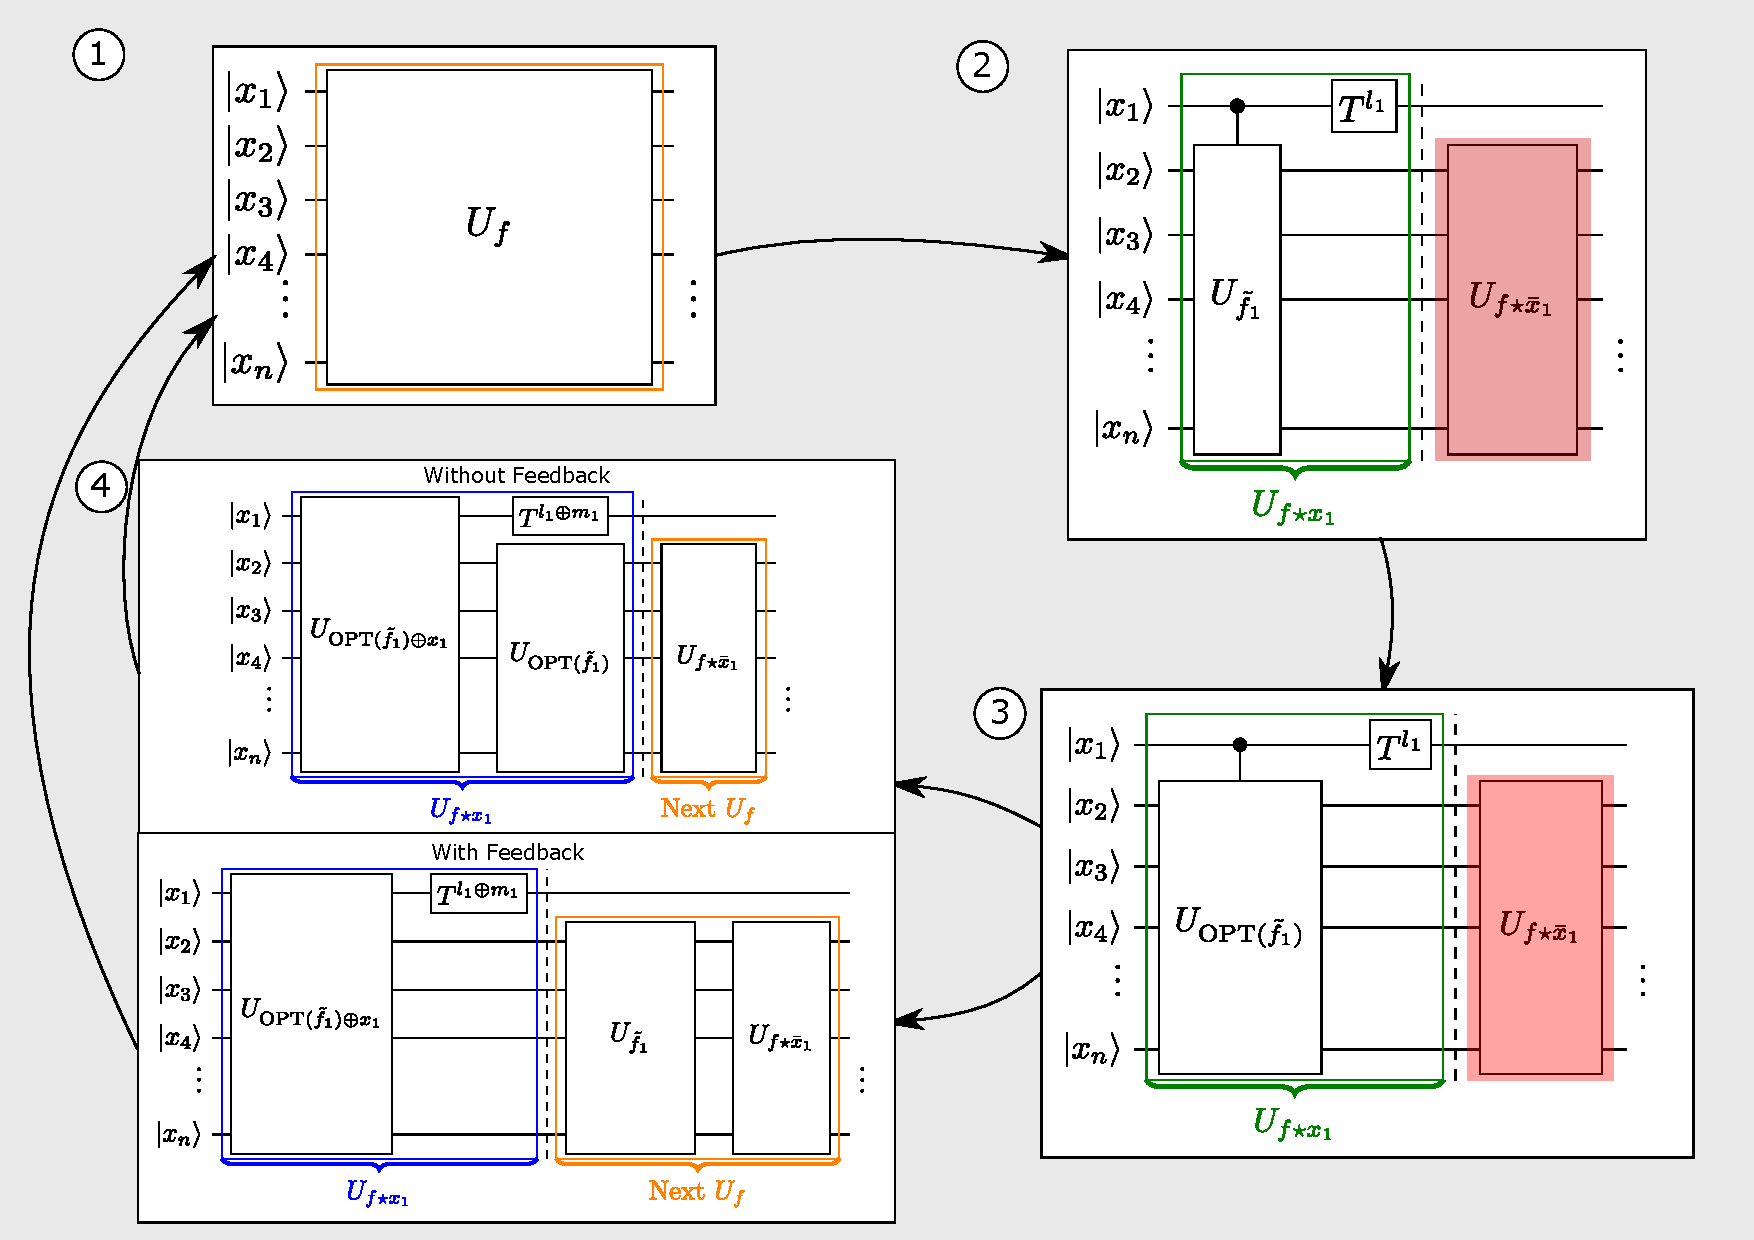
\includegraphics[width=0.7\linewidth]{TORfig3}
	\caption{The structure of the TOR algorithm is shown in the quantum circuit picture. The colours of each box have the following meanings: \textcolor{orange!80!black}{orange} border is for subcircuits yet to be pre-processed before the start of optimization and synthesis steps; \textcolor{green!50!black}{green} border shows subcircuits that are actively being optimized synthesized; \textcolor{blue}{blue} border is for synthesized subcircuits i.e. they are now decomposed into a sequence of CNOT and $T$ gates; and \textcolor{red}{red} fill are for subcircuits that not currently being processed.}
	\label{fig_TOR}
\end{figure}

We now describe a single round of optimization according to the TOOL algorithm. We begin by showing that given some input unitary $U_f \in \mathcal{D}_3$, we can decompose $U_f$ according to panel 2 of figure \ref{fig_TOR}. Recall the definition of the weighted polynomial from equation \ref{eq_wp},
\begin{equation}
f(\mathbf{x}) = \sum_{\alpha=1}^{n}l_{\alpha}x_\alpha + 2\sum_{\alpha<\beta}^{n} q_{\alpha,\beta}x_\alpha x_\beta + 4\sum_{\alpha<\beta<\gamma}^{n}c_{\alpha,\beta,\gamma}x_\alpha x_\beta x_\gamma \pmod{8}
\end{equation}
Now, we group terms in the following way,
\begin{equation}
\label{eq_TOR_decomp}
f(\mathbf{x}) = 2x_h\tilde{f}_{h}(\mathbf{x}\setminus x_h) + l_h x_h + f^\prime_{h}(\mathbf{x}\setminus x_h) \pmod{8},
\end{equation}
where we have defined the following:
\iffalse\begin{definition}{\textbf{Operators}: }
	Let $f(\mathbf{x})$ be a weighted polynomial on $n$ qubits.
	\begin{align}
	&f\star x_h = \text{weighted polynomial that consists of all the terms of $f$ that $x_h$ is a factor.}\\
	&f\star \bar{x}_h = \text{weighted polynomial that consists of all the terms of $f$ that $x_h$ is \emph{not} a factor.}\\
	&\tilde{f}_h = \frac{(f\star x_h) - l_h x_h}{2x_h}
	\end{align}
	\emph{Note: It follows that $f = f\star x_h + f\star \bar{x}_h$ and that $\tilde{f}_h\star x_h = 0$}
\end{definition}\fi
\begin{definition}{\textbf{Target Polynomial}. }
	Let $f(\mathbf{x})$ be a weighted polynomial on $n$ qubits. We say $\tilde{f}_{h}(\mathbf{x}\setminus x_h)$ is the target polynomial of $f$ with respect to $x_h$ defined such that
	\begin{align}	
	&\tilde{f}_{h} = \frac{f_{h}-f^\prime_{h}-l_h}{2},
	\end{align}
	where $f_{h}$ and $f^\prime_{h}$ are the positive and negative Shannon cofactors of $f$ with respect to $x_h$.	
\end{definition}
The first term in equation \ref{eq_TOR_decomp} corresponds to the control-$U_{\tilde{f}_{h}}$ in panel 2 of figure \ref{fig_TOR}, where in our example circuit $h=1$. The second term corresponds to the $T^{l_h}$ gate. The final term corresponds to the only operator to the right of the dotted line, $U_{f^\prime_{h}}$, which acts on $n-1$ qubits. The key part of this construction is that by factoring out $2x_h$ from a portion of $f$, we obtain a lower order target polynomial, $\tilde{f}_{h}$, that is only defined up to quadratic terms, or explicitly:
\begin{equation}
\tilde{f}_h(\mathbf{x}) = \sum_{\alpha=1, \alpha\neq h}^n q_{\alpha,h} x_\alpha + 2\sum_{\alpha<\beta,\beta\neq h}^{n}c_{\alpha,\beta,h}x_\alpha x_\beta \pmod{8}.
\end{equation}
Operators of the form control-$U_{\tilde{f}_{h}}$ are uniquely defined (up to Clifford equivalence) by a signature tensor of order 2, rather than order 3 as in the TODD algorithm (see section \ref{sec_TODD}). For a given target polynomial, $\tilde{f}_{h}$, we define the order 2 signature tensor (in a way analogous to equation \ref{eq_def_sig}) in terms of the coefficients of the original weighted polynomial, $f$,
% Define order 2 signature tensor problem.
%The signature tensor problem of order 2 has been solved efficiently by Lempel \cite{8_Lempel_1975}
\begin{align}
&S_{\alpha,\alpha} = q_{a,h} &&\pmod{2} \\
&S_{\alpha,\beta} = S_{\beta,\alpha} = c_{\alpha,\beta,h} &&\pmod{2},
\end{align}
which can be determined from a gate synthesis matrix, $A\in \mathbb{Z}_2^{(n,m)}$, that implements $\tilde{f}_h$,
\begin{equation}
\label{eq_sigTOR}
S_{\alpha,\beta} = \sum_{j=1}^{m}A_{\alpha,j}A_{\beta,j} \pmod{2}.
\end{equation}
The optimization step between panels 2 and 3 of figure \ref{fig_TOR} is to find an $A$ matrix with minimal columns that satisfies equation \ref{eq_sigTOR}.
\begin{problem}{\textbf{(2-STR)}}
	Given a symmetric tensor of order 2, $S\in \mathbb{Z}_2^{(n,n)}$, find a matrix $A \in \mathbb{Z}_2^{(n,m)}$ that satisfies equation \ref{eq_sigTOR} with minimal $m$.
\end{problem}
It turns out that this problem is exactly equivalent to the matrix factoring problem solved by Abraham Lempel in reference \cite{8_Lempel_1975}. In an effort to make this paper more self-contained, we provide a description of Lempel's algorithm in appendix \ref{ap_lempel}. For now, we treat Lempel's solver as a black box $OPT(\tilde{f})$ that outputs an optimized decomposition for the input target polynomial $\tilde{f}$, as can be seen in panel 3 of figure \ref{fig_TOR}.

% 1 Convert control-Optimized to CNOT + T's
% 2 Difference between feedback and without feedback
% 3 Repeat the cycle with new U_f. Each cycle reduces size of circuit
% 4 Finally use RM when small enough



\subsection{Third Order Duplicate and Destroy (TODD)}
\label{sec_TODD}
In this section, we present an algorithm based in principle on Lempel's matrix factoring algorithm \cite{8_Lempel_1975} that is extended to work for tensors of order 3. This algorithm requires some initial $A$ matrix to be generated by another algorithm such as RE or TOOL, then it reduces the number of columns of the initial gate synthesis matrix iteratively until exit. In section \ref{sec_results}, we present numerical evidence that it is the best efficient solver of the 3-STR problem developed so far.
\iffalse The algorithm works by identifying a subset of columns of an input gate synthesis matrix, $A$, to which we can add an arbitrary column vector, $\mathbf{z}$. This allows us to force pairs of columns to be identical, and identical columns can be removed without changing the unitary that it implements up to a Clifford factor\fi We call this the \emph{Third Order Duplicate and Destroy} (TODD) algorithm because, much like the villainous Victorian barber, it shaves away at the columns of the input $A$ matrix iteratively until the algorithm finishes execution.

\iffalse The rest of this section is consists of three parts: the first part shows that we can add an arbitrary column vector to a subset of columns of the gate synthesis matrix without altering the signature tensor. The second part shows that choosing a specific value of $\mathbf{z}$ results in a new gate synthesis matrix that has two identical columns, which can be subsequently eliminated. The third and final part describes the flow of the algorithm itself.\fi

We begin by introducing the key mechanism through which TODD reduces the $T$ count of quantum circuits: by \emph{destroying} pairs of duplicate columns of a gate synthesis matrix, a process which can be done without changing the signature tensor, as shown in the following lemma.
\theoremstyle{Lemma}
\begin{lemma}{}
	\label{lemma_1}
	Let $A\in \mathbb{Z}^{(n,m)}$ be a gate synthesis matrix whose $a$\textsuperscript{th} and $b$\textsuperscript{th} columns are duplicates and $A^\prime\in \mathbb{Z}^{(n,m-2)}$ be a gate synthesis matrix formed from by removing the $a$\textsuperscript{th} and $b$\textsuperscript{th} columns of $A$. It follows that $S^{(A)}=S^{(A^\prime)}$ for any such $A$ and $A^\prime$.
\end{lemma}
\begin{proof}
	We start by writing the signature tensor in terms of the elements of $A$ according to equation \ref{eq_sig},
	\begin{equation}
	S^{(A)}_{\alpha,\beta,\gamma} = \sum_{k=1}^{m}A_{\alpha,k}A_{\beta,k}A_{\gamma,k} \pmod{2},
	\end{equation}
	and separating the terms associated with $a,b$ from the rest of the summation,
	\begin{equation}
	\label{proof_1_2}
	S^{(A)}_{\alpha,\beta,\gamma} = \sum_{j\in \mathcal{J}}A_{\alpha,j}A_{\beta,j}A_{\gamma,j} + A_{\alpha,a}A_{\beta,a}A_{\gamma,a} + A_{\alpha,b}A_{\beta,b}A_{\gamma,b} \pmod{2},
	\end{equation}
	where $\mathcal{J} = \left[1,m\right]\setminus \{a, b\}$.
	As stated in the lemma, the $a$\textsuperscript{th} and $b$\textsuperscript{th} columns of $A$ are duplicates and so
	\begin{equation}
		\label{proof_1_3}
		A_{i,a} = A_{i,b}\ \forall\ i \in \left[1,n\right].
	\end{equation}
	Now substitute equation \ref{proof_1_3} into equation \ref{proof_1_2},
	\begin{align}
	S^{(A)}_{\alpha,\beta,\gamma} &= \sum_{j\in \mathcal{J}}A_{\alpha,j}A_{\beta,j}A_{\gamma,j} + A_{\alpha,a}A_{\beta,a}A_{\gamma,a} + A_{\alpha,a}A_{\beta,a}A_{\gamma,a} \pmod{2}\\
	&= \sum_{j\in \mathcal{J}}A_{\alpha,j}A_{\beta,j}A_{\gamma,j} \pmod{2}\\
	&= S^{(A^\prime)}_{\alpha,\beta,\gamma},
	\end{align}
	where the penultimate step follows from modulo 2 addition and the final step follows from the definition of $A^\prime$ and equation \ref{eq_sig}.
\end{proof}
Lemma \ref{lemma_1} gives us a simple means to remove columns from a gate synthesis matrix by destroying pairs of duplicates columns and thereby reducing the $T$ count of a CNOT + $T$ circuit by 2. However, it is often the case that the $A$ matrix does not already contain any duplicate columns. Therefore, we wish perform some transformation on the $A$ matrix, which results in a different gate synthesis matrix $A^\prime$ that: a) has duplicate columns; b) preserves the signature tensor of $A$; and c) does not increase the column number of $A$ by more than 1. In the following lemma we introduce a class of transformations that \emph{duplicate} a particular column of an $A$ matrix such that properties a) and c) are met. We then use lemma \ref{lem1} establish what conditions must be satisfied for the duplication transformation to have property b).

\theoremstyle{lemma}
\begin{lemma}{}
	\label{lem2}
	Let $A$ be an $n\times m$ gate synthesis matrix where all columns are unique and non-zero. Let $A^\prime = A \oplus \mathbf{z}\mathbf{y}^T$ where $\mathbf{z}$ and $\mathbf{y}$ are column vectors on $\mathbb{Z}_2$ of length $n$ and $m$, respectively, defined such that $z_i = A_{i,a} \oplus A_{i,b}$ for some $a,b\in \left[1,m\right]$ and $y_a \oplus y_b = 1$. It follows that the $a$\textsuperscript{th} and $b$\textsuperscript{th} columns of $A^\prime$ are duplicates.
\end{lemma}
\begin{proof}
	We begin the proof by finding expressions for the matrix elements of $A^\prime$ in terms of $A$, $\mathbf{z}$ and $\mathbf{y}$,
	\begin{equation}
	A^\prime_{i,j} = A_{i,j} \oplus z_i y_j,
	\end{equation}
	and substitute the definition of $\mathbf{z}$,
	\begin{equation}
	A^\prime_{i,j} = A_{i,j} \oplus (A_{i,a}\oplus A_{i,b}) y_j.
	\end{equation}
	Now we can find the elements of the columns $a$ and $b$ of $A^\prime$,
	\begin{align}
	A^\prime_{i,a} &= A_{i,a} \oplus (A_{i,a}\oplus A_{i,b}) y_a,\\
	A^\prime_{i,b} &= A_{i,b} \oplus (A_{i,a}\oplus A_{i,b}) y_b.
	\label{e_working2}
	\end{align}
	We substitute in the condition $y_b = y_a \oplus 1$ into \ref{e_working2},
	\begin{align}
	\begin{split}
	A^\prime_{i,b} &= A_{i,b} \oplus (A_{i,a}\oplus A_{i,b}) (y_a \oplus 1) \\
	%&= A_{i,b} + (A_{i,a}+A_{i,b})y_a + A_{i,a}+A_{i,b} \\
	&= A_{i,a} \oplus (A_{i,a}\oplus A_{i,b})y_a \\
	& = A^\prime_{i,a}.
	\end{split}			
	\end{align}
\end{proof}

		\iffalse Let $\mathcal{I} = \{\left(\alpha,\beta,\gamma\right)\mid 1 \leq \alpha \neq \beta \neq \gamma \leq n\}$ be the set of all 3-tuples such that each element falls in the range $\left[1,n\right]$ and is unique. We define $\chi(A,x)$ to be an $|\mathcal{I}| \times m$ matrix that is a function of $A$ and $x$, an $n \times m$ matrix and a column vector of length $n$, respectively:
		\begin{equation}
		\label{e_chi}
		\left(\chi(A,x)\right)_{i,j} = x_\alpha A_{\beta,j} A_{\gamma,j} + x_\beta A_{\gamma,j} A_{\alpha,j} + x_\gamma A_{\alpha,j} A_{\beta,j},
		\end{equation}
		where $\left(\alpha,\beta,\gamma\right)$ is the $i^\text{th}$ element of $\mathcal{I}$. \fi
		
		\theoremstyle{lemma}
		\begin{lemma}{}
			\label{lem1}
			Let $A$ and $A^\prime = A \oplus \mathbf{z}\mathbf{y}^T$ be two gate synthesis matrices where $\mathbf{z}$, $\mathbf{y}$ are arbitrary column vectors of dimension $n$ and $m$, respectively. $S^{(A)} = S^{(A^\prime)}$ as long as the following conditions hold true:
			\begin{enumerate}
				\item [C1:] $\quad |\mathbf{y}| = 0\pmod{2}$
				\item [C2:] $\quad A\mathbf{y} = \mathbf{0}$
				\item [C3:] $\quad \chi(A,\mathbf{z})\hspace{1mm}\mathbf{y} = \mathbf{0}$.
			\end{enumerate}
			where we define $\chi(A,\mathbf{z})$ as follows:
			\begin{definition}{\textbf{$\chi$ Matrix.}}
				Given some gate synthesis matrix, $A$, and a column vector $\mathbf{z}\in\mathbb{Z}_2^n$ let					
				\begin{equation*}
				\chi(A,\mathbf{z}) = \normalsize\begin{pmatrix}
				(z_1\mathbf{r_2}\wedge\mathbf{r_3})\oplus (z_2\mathbf{r_3}\wedge\mathbf{r_1})\oplus (z_3\mathbf{r_1}\wedge\mathbf{r_2})\\
				(z_1\mathbf{r_2}\wedge\mathbf{r_4})\oplus (z_2\mathbf{r_4}\wedge\mathbf{r_1})\oplus (z_4\mathbf{r_1}\wedge\mathbf{r_2})\\
				\vdots \\
				(z_{n-2}\mathbf{r_{n-1}}\wedge\mathbf{r_{n}})\oplus (z_{n-1}\mathbf{r_{n}}\wedge\mathbf{r_{n-2}})\oplus (z_{n}\mathbf{r_{n-2}}\wedge\mathbf{r_{n-1}})\\
				\end{pmatrix}\large,
				\end{equation*}
				where $\mathbf{r_i}$ is the $i^{\text{th}}$ row of $A$, and $\mathbf{x}\wedge\mathbf{y}$ is the element-wise product of vectors $\mathbf{x}$ and $\mathbf{y}$.
			\end{definition}
		\end{lemma}
		\begin{proof}
			We begin the proof by finding an expression for $S(A^\prime)$ using equation \ref{eq_sig},
			\begin{equation}
			S^{(A^\prime)}_{\alpha,\beta,\gamma} = \sum_{j=1}^{m}\left(A_{\alpha,j}\oplus z_\alpha y_j\right)\left(A_{\beta,j}\oplus z_\beta y_j\right)\left(A_{\gamma,j}\oplus z_\gamma y_j\right) \pmod{2},
			\end{equation}
			and expanding the brackets,
			\begin{align}
			\label{e_working1}
			\begin{split}
			S^{(A^\prime)}_{\alpha,\beta,\gamma} = \sum_{j=1}^{m}(&A_{\alpha,j}A_{\beta,j}A_{\gamma,j} \oplus z_\alpha z_\beta z_\gamma y_j  \\			
			&\oplus z_\alpha z_\beta A_{\gamma,j} y_j \oplus z_\beta z_\gamma A_{\alpha,j} y_j \oplus z_\gamma z_\alpha A_{\beta,j} y_j \\
			&\oplus z_\alpha A_{\beta,j} A_{\gamma,j} y_j \oplus z_\beta A_{\gamma,j} A_{\alpha,j} y_j \oplus z_\gamma A_{\alpha,j} A_{\beta,j} y_j) \pmod{2}.
			\end{split}
			\end{align}
			We can see that the first term of equation \ref{e_working1} summed over all $j$ is equal to $S^{(A)}$, by definition. The task is to show that the remaining terms sum to zero under the specified conditions. Next, we sum over all $j$ and substitute in the definitions of $|\mathbf{y}|$, $A\mathbf{y}$ and $\chi(A,\mathbf{z})\hspace{1mm}\mathbf{z}$,
			\begin{equation}
			S^{(A^\prime)}_{\alpha,\beta,\gamma} = S^{(A)}_{\alpha,\beta,\gamma} \oplus z_\alpha z_\beta z_\gamma |\mathbf{y}| \oplus z_\alpha z_\beta \left[A\mathbf{y}\right]_\gamma \oplus z_\beta z_\gamma \left[A\mathbf{y}\right]_\alpha \oplus z_\gamma z_\alpha \left[A\mathbf{y}\right]_\beta \oplus \left[\chi(A,\mathbf{z})\hspace{1mm}\mathbf{y}\right]_{\iota(\alpha,\beta,\gamma)},
			\end{equation}
			where we $\iota(\alpha,\beta,\gamma)$ is the row index of $\chi$ whose elements are given by $(z_\alpha\mathbf{r_\beta}\wedge\mathbf{r_\gamma})\oplus (z_\beta\mathbf{r_\gamma}\wedge\mathbf{r_\alpha})\oplus (z_\gamma\mathbf{r_\alpha}\wedge\mathbf{r_\beta})$.		
			By applying condition \emph{C1}, the second term is eliminated; by applying condition \emph{C2}, the next three terms are eliminated, and by applying condition \emph{C3}, the final term is eliminated.
		\end{proof}
	
		\begin{algorithm}		
				\caption{Third Order Duplicate-then-Destroy (TODD) Algorithm}
				\label{al_1}
				\textbf{Input:} Gate synthesis matrix $A\in \mathbb{Z}_2^{(n,m)}$. \\
				\textbf{Output:} Gate synthesis matrix $A^\prime \in \mathbb{Z}_2^{(n,m^\prime)}$ such that $m^\prime \leq m$ and $S^{(A^\prime)}=S^{(A)}$.
				\footnotesize
				\begin{itemize}
					\item Let $\mathrm{col}_j(A)$ be a function that returns the $j^{\text{th}}$ column of $A$.
					\item Let $\text{cols}(A)$ be a function that returns the number of columns of $A$.
					\item Let $\text{nullspace}(A)$ be a function that returns a matrix whose columns generate the right nullspace of A.
					\item Let $\mathrm{simplify(A)}$ be a function that removes every pair of identical columns and every all-zero column from $A$.
				\end{itemize}
				\normalsize
				%\\Let $\text{col}_j(A)$ denote the $j^{\text{th}}$ column of $A$.
				\begin{algorithmic}			
					\Procedure{TODD}{}
					\State{Initialize $A^\prime \leftarrow A$}
					\BState \emph{start}:
					\ForAll{$1\leq a < b \leq \mathrm{cols}(A^\prime)$}
					%\State{\emph{Iterate over all column pairs.}}
					\State{$\mathbf{z}\leftarrow \text{col}_a(A^\prime) + \text{col}_b(A^\prime)$}
					\State{$\tilde{A}\leftarrow \begin{pmatrix}
						A^\prime \\%\hline			
						\chi(A^\prime,\mathbf{z})
						\end{pmatrix}$}
					\State{$N\leftarrow \text{nullspace}(\tilde{A})$}			
					\ForAll{$1 \leq k \leq \text{cols}(N)$}
					\State{$\mathbf{y}\leftarrow\text{col}_k(N)$}
					\If{$y_a\oplus y_b=1$}
					%\State{\emph{At least one column can be eliminated.}}
					\If{$|\mathbf{y}|=1 \pmod 2$}
					%\State{\emph{Force $y$ to be even weight and adjust width of $A^\prime$.}}
					\State{$A^\prime \leftarrow \begin{pmatrix}
						A^\prime & \mathbf{0}
						\end{pmatrix}$}
					\State{$\mathbf{y}\leftarrow \begin{pmatrix}
						\mathbf{y} \\
						1
						\end{pmatrix}$}					
					\EndIf
					\State{$A^\prime \leftarrow A^\prime + \mathbf{z}\mathbf{y}^T$}
					\State{$\mathrm{simplify(A^\prime)}$}
					\State{\textbf{goto} \emph{start}}
					\EndIf
					\EndFor
					\EndFor
					\EndProcedure			
				\end{algorithmic}
			\end{algorithm}
	
		Now we have shown how to duplicate and destroy columns of a gate synthesis matrix, we are ready to describe the TODD algorithm, presented as pseudo-code in algorithm \ref{al_1}. Given an input gate synthesis matrix $A$ with signature tensor $S$, we begin by iterating through all column pairs of $A$ given by indices $a,b$. We construct the vector $\mathbf{z}=\mathbf{c}_a \oplus \mathbf{c}_b$ where $\mathbf{c}_j$ is the $j$\textsuperscript{th} column of $A$, as in lemma \ref{lem2}. We check to see if the conditions in lemma \ref{lem1} are satisfied for $\mathbf{z}$ by forming the matrix,
		\begin{equation}
		\tilde{A}=\begin{pmatrix}
		A \\ \chi(A,\mathbf{z})
		\end{pmatrix}.
		\end{equation}
		Any vector, $\mathbf{y}$, in the null space of $\tilde{A}$ simultaneously satisfies \emph{C2} and \emph{C3} of lemma \ref{lem1}. We scan through the null space basis until we find a $\mathbf{y}$ such that $y_a \oplus y_b = 1$. At this stage we know that we can remove at least one column from $A$. If $|\mathbf{y}|=0 \pmod{2}$ then condition \emph{C1} is satisfied and we can perform the duplication transformation from lemma \ref{lem1}. Otherwise, we force \emph{C1} to be satisfied by appending a 1 to $\mathbf{y}$ and an all-zero column to $A$ before applying the duplication transformation. Finally, we duplicate columns by adding the value of $\mathbf{z}$ to every column $j$ for which $y_j = 1$, then destroy the $a$\textsuperscript{th} and $b$\textsuperscript{th} columns of $A$. This reduces the number of columns of $A$ and therefore the $T$ count of $U_f$. We now start again from the beginning, iterating over columns of the new $A$ matrix. The algorithm terminates if every column pair has been exhausted without success.		

		

	%\subsection{Computational Efficiency}
	
	\section{Results \& Discussion}
	\label{sec_results}
	We implemented our $T$ gate optimization protocol in C++ and ran it on two types of benchmark. First, we performed a random benchmark, in which we randomly sampled signature tensors from a uniform probability distribution for a range of $n$ and used them as input for four versions of \emph{T-optimiser}: RE, TOOL (feedback), TOOL (without feedback) and TODD. The results for the random benchmark are shown in figure \ref{fig_random}. Second, we tested the protocol on a library of benchmark circuits taken from Maslov's Reversible Logic Synthesis Benchmarks Page \cite{37_Maslov_web}. These circuits implement useful quantum algorithms including Galois Field multipliers, integer addition, n\textsuperscript{th} prime, Hamming coding functions and the hidden weighted bit functions. Some of these circuits feature the generalised ($n$-bit) Toffoli gate, which we implement in the Clifford + $T$ gate set using ancillas with a standard method \cite{35_Nielsen:2011:QCQ:1972505}. The results for the quantum algorithm benchmark are listed in table \ref{tab_CliffT}.
	
	\subsection{Random Benchmark}

	\begin{wrapfigure}{r}{0.47\linewidth}
		\centering
		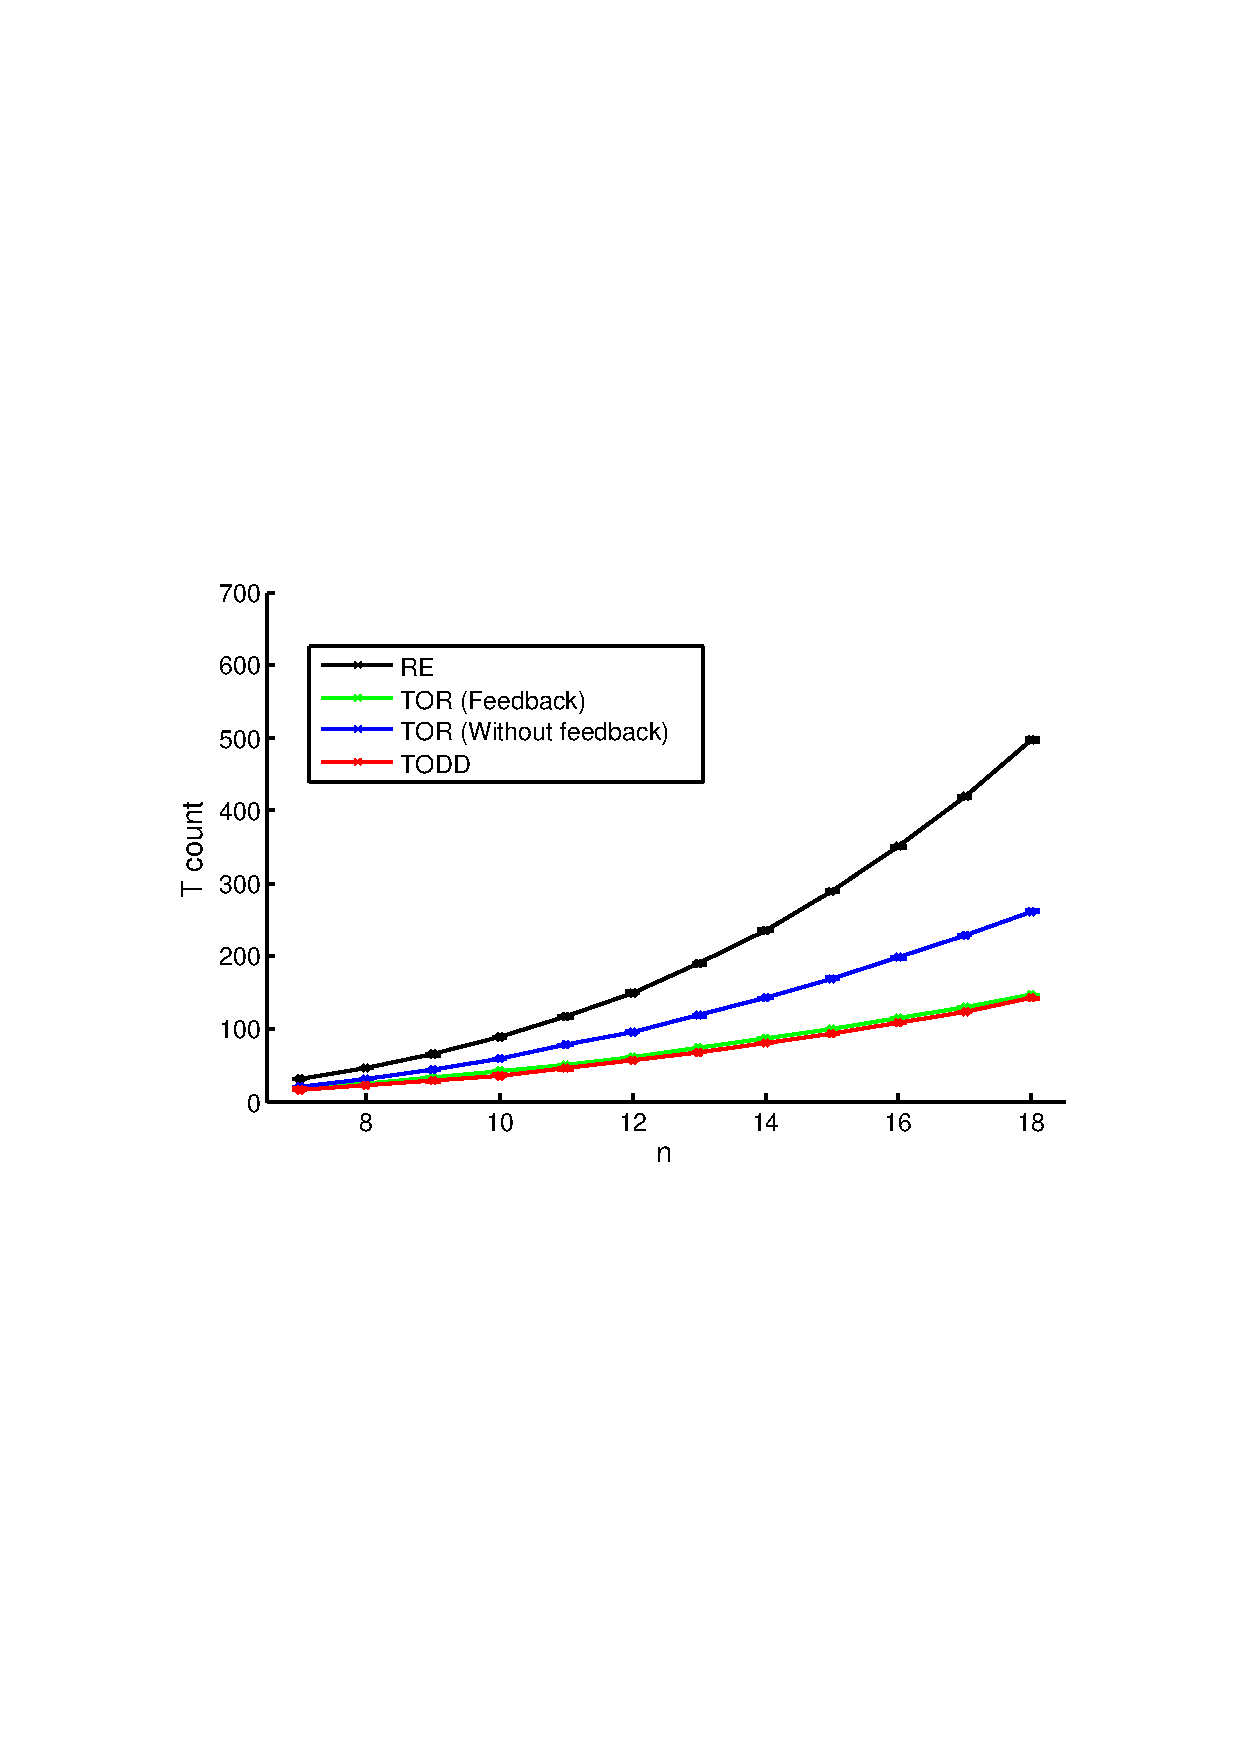
\includegraphics[width=\linewidth, trim={3cm 10cm 3cm 9.5cm},clip]{random_benchmark}
		\caption{\iffalse Circuits generated by the $\mathrm{CNOT}$ and $T$ gate were randomly generated for varying number of qubits $n$ then optimized by our implementations of RE, TOR and TODD. The average $T$-count for each $n$ over many random circuits are shown on the vertical axis. TODD produces circuit decompositions with the smallest $T$-counts on average but scales the same as the next best algorithm, TOR (Feedback). Both of these algorithms are better than RE by a factor $n$. The difference between the $T$-counts for TODD and TOR (Feedback) converge on a constant $5.5\pm 0.7$ for large $n$. 
		%BLAH repetitions were performed for each value of $n$.
		\fi
		Random benchmark.
		}
		\label{fig_random}
	\end{wrapfigure}
	
	We performed the random benchmark in order to determine the average case scaling of the $T$-count with respect to $n$ for each computationally efficient version of \emph{T-optimize}. 		For both versions of TOOL, we find that the numerical results for the $T$ count follows the expected analytical scaling of $\mathcal{O}(n^2)$ and correspondingly the results for RE scales as $\mathcal{O}(n^3)$.
	We see that TODD outperforms the next best algorithm, TOOL (without feedback), by a constant value of $5.5\pm0.7$ and is therefore the preferred algorithm in settings where classical runtime is not an issue.

	While both have a runtime of $\mathcal{O}(\mathrm{POLY}(n))$, the order of the polynomial is much higher for TODD than for TOOL. This means the latter would be preferable for some experimental settings where very large non-Clifford circuits must be generated within a limited time frame e.g. due to decoherence. But at this stage where the disparity between quantum and classical resource costs is so high, reducing the $T$ count is more important than reducing the classical runtime.
 	
	The random benchmark effectively benchmarks on random diagonal CNOT + T circuits. This gate set is not universal and therefore is computationally limited. However, these circuits are generated by $\{T, CS, CCZ\}$, which all commute. This means such circuits lie in the computational complexity class IQP (which stands for \emph{instantaneous quantum  polynomial-time}) that feature in proposals for quantum supremacy experiments \cite{2_Bremner_2010,monty,Shepherd1413}.  Low cost designs of IQP circuits provided by our protocol would therefore be an asset for achieving quantum supremacy.
	
	
	%We find the scaling for TOOL is quadratic as expected from the analytical argument.
	
	
	%Lastly, we tested the protocol on a number of single target gates generated by RevKit.
	
	%in order to achieve two goals: first benchmark test our different \emph{T-Optimise} algorithms against one another using random circuits (see figure \ref{fig_random}); and second to evaluate the performance of the full Clifford + $T$ protocol against the best known circuit decompositions for useful quantum algorithms, the results of which are listed in table \ref{tab_CliffT}. We see from both results that TODD produces quantum circuits with smallest $T$ count.
	
	%Intro paragraph
	%- Programming language
	%- Types of benchmark circuits
	%- Names of the algorithms computed
	%- Specification of computer used
	%- Processor: Clock speed, Type
	%- RAM: Amount, Type
	%- OS: Name, Version
	%- Verified by matrices (functional equivalence)
	%- Only for small test circuits
	
	

	
	\FloatBarrier
	
	\begin{table}[h!]
		\footnotesize
		\centering		
		%\caption{$T$-counts for various universal Clifford + $T$ benchmark circuits as synthesized by the TODD and RE algorithm are shown. $T_{\text{original}}$ are the best known results produced by the works cited in the \emph{Circuit} column, and $T_{\text{TODD}}$ is the result for TODD. \textbf{$n_{\text{original}}$} is the number of qubits of the original circuit and \textbf{$n_{\text{out}}$} is the total number of qubits of the output circuit including ancillas used to implement multiply controlled Toffoli gates as well as Hadamards using path variables \cite{1_Montanaro_2017}. The total execution time in seconds for TODD run on an \emph{Intel i7} 2.40Gz processor is given in column \emph{Time}.}
		\iffalse\begin{tabular}{ |>{\columncolor{white}}l|>{\columncolor{blue!25}}r|>{\columncolor{green!25}}r|>{\columncolor{gray!10}}r|>{\columncolor{white}}r|>{\columncolor{gray!10}}r|>{\columncolor{white}}r| }					
			\hline						
			\rowcolor{gray!25}
			\textbf{Circuit} & \textbf{$T_{\text{original}}$} & \textbf{$T_{\text{TODD}}$} & \textbf{$T_{\text{RE}}$} & \textbf{$n_{\text{original}}$} & \textbf{$n_{\text{out}}$} & \textbf{Time (s)} \\
			\hline						
			hwb6\_47\_107 \cite{3_Amy_2016} & 71 & 55 & 102 & 6 & 43 & 91.713 \\
			hwb6-42-150 \cite{3_Amy_2016} & 71 & 46 & 140 & 6 & 43 & 160.198 \\
			nth\_prime6\_inc\_55\_667 \cite{3_Amy_2016} & 400 & 263 & 354 & 6 & 39 & 228.025 \\
			ham15-109-214 \cite{3_Amy_2016} & 97 & 28 & 65 & 15 & 47 & 27.756 \\
			ham15-70 \cite{3_Amy_2016} & 230 & 103 & 148 & 15 & 47 & 100.899 \\
			ham15tc1 \cite{3_Amy_2016} & 1019 & 258 & 359 & 15 & 50 & 270.862 \\
			\emph{$^\#$0117} \cite{41_soeken} & 79 & 13 & 63 & 6 & 116 & 118.64 \\
			\emph{$^\#$017F} \cite{41_soeken} & 80 & 23 & 59 & 6 & 59 & 20.618 \\
			\emph{$^\#$0001} \cite{41_soeken} & 40 & 21 & 46 & 6 & 39 & 5.2 \\
			\emph{$^\#$001F} \cite{41_soeken} & 43 & 22 & 55 & 6 & 39 & 4.382 \\
			\emph{$^\#$0007} \cite{41_soeken} & 47 & 13 & 31 & 6 & 64 & 10.141 \\
			\emph{$^\#$007F} \cite{41_soeken} & 40 & 19 & 46 & 6 & 27 & 1.267 \\
			GF$(2^4)$-Mult & 68 & 50 & 68 & 12 & 19 & 3.79 \\
			GF$(2^5)$-Mult & 101 & 90 & 115 & 15 & 24 & 45.142 \\
			GF$(2^6)$-Mult & 144 & 134 & 150 & 18 & 29 & 307.051 \\
			GF$(2^7)$-Mult & 208 & 173 & 197 & 21 & 34 & 896.94 \\
			GF$(2^8)$-Mult & 237 &  &  &  &  & \\
			RC-Adder\textsubscript{6} & 77 & 36 & 49 & 14 & 51 & 33.963 \\
			\hline
		\end{tabular}\fi
		\caption{$T$-counts for Clifford + $T$ benchmarks circuits. We show the number of qubits $n$ and the $T$-count for the circuit: before optimization (pre-opt.);  after optimization (post-opt.) using the best previous algorithm; and post-optimization using our implementation of TODD. We show the $T$-count saving for TODD over the best previous algorithm, as well as the total execution time.}
		\begin{tabularx}{0.85\textwidth}{|X|cc|ccc|cccc|}
		\hline
		\multirow{2}{*}{\textbf{Circuit}} & \multicolumn{2}{c|}{\textbf{Pre-Opt.}} & \multicolumn{3}{c|}{\textbf{Post-Opt. (Best Prev.)}} & \multicolumn{4}{c|}{\textbf{Post-Opt. (TODD)}} \\
		& \textbf{n} & \textbf{T} & \textbf{n} & \textbf{T} & \textbf{Due to} & \textbf{n} & \textbf{T} & \textbf{\scriptsize Saving (\%)} & \textbf{Runtime (s)} \\
		\hline
		%4-bit adder & 5 & 28 & 5 & 16 & T-par & 10 & 16 & 0 & 0.016 \\
		8-bit adder & 24 & 350 & 24 & 213 & RM(maj) & 108 & 49 & 77.00 & 506.193 \\		
		GF($2^4$)-mult & 12 & 112 & 12 & 68 & T-par & 19 & 50 & 26.47 & 5.408 \\
		GF($2^5$)-mult & 15 & 175 & 15 & 111 & T-par & 24 & 97 & 12.61 & 43.822 \\
		GF($2^6$)-mult & 18 & 252 & 18 & 150 & T-par & 29 & 136 & 9.333 & 259.38 \\
		GF($2^7$)-mult & 21 & 343 & 21 & 217 & T-par & 34 & 176 & 18.89 & 1869.24 \\		
		HWB$_6$ & 7 & 105 & 7 & 71 & T-par & 41 & 45 & 36.62 & 67.11 \\
		QCLA-Adder$_{10}$ & 36 & 238 & 36 & 162 & T-par & 64 & 59 & 63.58 & 123.55 \\
		QCLA-COM$_7$ & 24 & 203 & 24 & 94 & RM(maj)	& 56 & 35 & 62.77 & 52.006	\\
		QCLA-Mod$_7$ & 26 & 413 & 26 & 235 & Auto (H) & 98 & 58 & 75.32 & 989.694 \\
		RC-Adder$_6$ & 14 & 77 & 14 & 47 & RM(maj/rec) & 51 & 36 & 23.40 & 37.866 \\
		VBE-Adder$_3$ & 10 & 70 & 10 & 24 & T-par & 14 & 20 & 16.67 & 0.101 \\
		Grover$_5$ & 9 & 336 & 9 & 52 & T-par & 127 & 39 & 25.00 & 452.677 \\
		CSLA-MUX$_3$ & 15 & 70 & 15 & 58 & RM(rec) & 32 & 50 & 13.79 & 15.563 \\
		CSUM-MUX$_9$ & 30 & 196 & 30 & 76 & RM(rec) & 81 & 36 & 52.63 & 74.525 \\
		Mod-Red$_{21}$ & 11 & 119 & 11 & 73 & T-par & 36 & 50 & 31.51 & 15.52 \\
		Mod-Mult$_{55}$ & 9 & 49 & 9 & 35 & RM(maj/rec) & 32 & 34 & 2.857 & 4.904 \\
		Hamming$_{15}$ (low) & 17 & 161 & 17 & 97 & T-par & 51 & 34 & 64.95 & 45.282 \\
		Hamming$_{15}$ (med) & 17 & 574 & 17 & 230 & T-par & 102 & 49 & 78.70 & 796.282 \\
		QFT$_4$ & 5 & 69 & 5 & 67 & T-par & 44 & 37 & 44.78 & 19.547 \\
		NC Toff$_4$ & 4 & 21 & 4 & 15 & T-par & 7 & 13 & 13.33 & $<0.001$ \\
		NC Toff$_5$ & 5 & 35 & 5 & 23 & T-par & 11 & 20 & 13.04 & 0.046 \\
		NC Toff$_6$ & 6 & 49 & 6 & 31 & T-par & 15 & 25 & 19.36 & 0.199 \\
		NC Toff$_{10}$ & 11 & 119 & 11 & 71 & T-par & 35 & 46 & 35.21 & 10.877 \\
		\hline\multicolumn{6}{c|}{} & \multicolumn{2}{l}{\cellcolor{lightgray}\textbf{Average}} & \cellcolor{lightgray}\textbf{34.08} & \cellcolor{lightgray} \\
		\multicolumn{6}{c|}{} & \multicolumn{2}{l}{\cellcolor{lightgray}\textbf{Max}} & \cellcolor{lightgray}\textbf{78.70} & \cellcolor{lightgray} \\ \cline{7-10}				
		\end{tabularx}
		\label{tab_CliffT}		
	\end{table}
	
	\subsection{Quantum Algorithms}

	The results in table \ref{tab_CliffT} show us that TODD successfully reduced the $T$ count for every algorithm upon which it was tested and has an average and maximum saving of $34\%$ and $79\%$, respectively. This is immediately useful due to the lower cost associated with solving these problems. However, we acknowledge that the $T$ count does not account for the full space-time cost of quantum computation (often referred to as the aggregate cost). In this work, we ignore the cost of Clifford gates due to the high ratio between the aggregate cost of the $T$ gate and that of Clifford gates. The aggregate cost is highly sensitive to the architecture of the quantum computer, but for the surface code, this ratio is estimated to be between 100 and 1000 \cite{raus,ogor,fowl}.

While our protocol leads to circuits with low $T$ count, the final output often has an \emph{increased} CNOT count. This is due to step 6 of our protocol where we map the phase polynomial back to a quantum circuit using a naive approach. As our work concerns $T$ gate optimization, we leave the problem of optimizing CNOT count as an avenue for further work.

	\section{Conclusions}
	\label{s_d_and_c}
	In this work, we have outlined a framework for optimizing large Clifford + $T$ quantum circuits such that the output has $T$ count near the global optimum and the run time is polynomial in both the number of qubits and the number of gates. This scheme maps the quantum circuit problem to a problem on order 3 symmetric tensors. We have presented an efficient near-optimal approach for solving this problem and reviewed previous methods. We implemented our protocol in C++ and used it to produce circuit decompositions for quantum algorithms with lower $T$-counts than any previous attempt known to the best of our knowledge. This lowers the cost of quantum computation and takes us closer to the common goal of achieving practical universal fault-tolerant quantum computation.
	

	\section{Acknowledgements}
	We acknowledge support by the Engineering and Physical Sciences Research Council (EPSRC) (Grant No. EP/M024261/1). We thank Mark Howard and Matthew Amy for valuable discussions.
	%F Acknowledgements
	%- EPSRC Funded
	%- Matthew Amy (useful emails), Mark Howard (discussions), Padraic, Mike, Joscka (conversations)

	\bibliographystyle{ieeetran}
	%\bibliographystyle{abbrv}
	\bibliography{lempelx_lit}
	
	\appendix
	\section{Lempel's Factoring Algorithm}
	\label{ap_lempel}
	We describe Lempel's factoring algorithm (originally from reference \cite{8_Lempel_1975}) using conventions consistent with our description of the TODD algorithm to more easily see how TODD generalizes Lempel's algorithm for order 3 tensors.

	Lempel's factoring algorithm takes as input a symmetric tensor of order 2 (a matrix), which we denote $S\in \mathbb{Z}_2^{(n,n)}$ and outputs a matrix $A\in \mathbb{Z}_2^{(n,m)}$ where the elements of $A$ and $S$ are related as follows:
	\begin{equation}
		\label{eq_lemp1}
		S_{\alpha,\beta} = \sum_{k=1}^{m}A_{\alpha,k}A_{\beta,k} \pmod{2}.
	\end{equation}
	In reference \cite{8_Lempel_1975}, Lempel proves that the minimal value of $m$ is equal to
	\begin{equation}
	\mu(S) = \rho(S) + (1 \oplus \vee_i^nS_{i,i}),
	\end{equation}
	where $\rho(S)$ is the rank of matrix $S$ and $\vee$ is the logical OR operator.
	 Lempel's algorithm solves the problem of finding an $A$ matrix that obeys equation \ref{eq_lemp1} for a given $S$ matrix such that $m=\mu(S)$. Such an $A$ matrix is referred to as a minimal factor of $S$. 
		
	In the following, we denote the number of columns of $A$ as $c(A)$, the $j$\textsuperscript{th} column of $A$ as $c_j(A)$. Lempel's algorithm consists of the following 7 steps:
	\begin{enumerate}
		\item Generate an initial (necessarily suboptimal) $A$ matrix for $S$.
		\item Check if $c(A) = \mu(S)$. If true, exit and output $A$. Otherwise, perform steps 3 to 7.
		\item Find a $y\in\mathbb{Z}_2^m$ such that $Ay = \mathbf{0}$ and $\vee_i^m(y_{i}\oplus 1)=1$.
		\item If $|y|=1 \pmod{2}$ then update $y \rightarrow (y^T, 1)^T$ and $A = (A \quad \mathbf{0})$.
		\item Find a pair of indices $a,b\in [1,m], \ a\neq b$ such that $y_a \oplus y_b = 1$.
		\item Apply transformation $A \rightarrow A \oplus zy^T$, where $z=c_a(A) \oplus c_b(A)$.
		\item Remove columns $a$ and $b$ from $A$, then go to step 2.
	\end{enumerate}

	The above algorithm is designed to work for the special case where the input $S$ matrix is non-singular. However, Lempel provides a means of extending to the singular case using a pre-processing step on the input $S$ matrix:
	\begin{equation}
	\tilde{S} = RSR^T = \begin{pmatrix}
	S^\prime & 0 \\ 0 & 0
	\end{pmatrix},
	\end{equation}
	where $S^\prime$ is a non-singular symmetric matrix with $\rho(S)$ rows. The matrix $R$ is constructed as follows:
	\begin{equation}
	R = LP,
	\end{equation}
	where $P$ is a permutation matrix such that the first $\rho(S)$ rows of $PS$ are linearly independent and $L$ is a self-inverse lower diagonal matrix such that the last $n-\rho(S)$ rows of $TPSP^T$ are all zero vectors.
	Lempel's algorithm is performed on $S^\prime$ to obtain a minimal factor $A^\prime$. Finally, we recover the minimal factor of $S$ by applying the transformation:
	\begin{equation}
	A = P^TT\begin{pmatrix}
	A^\prime \\ 0
	\end{pmatrix}.
	\end{equation}
	%There's a bit more stuff for non-singular $S$ matrices but I haven't written that yet.
	%Check if Lempel's paper explains why this algorithm always terminates.
	
	\section{Calculating $\mathcal{U}_{\text{Clifford}}^\dagger$}
	\label{ap_Cliff}
	We will now describe how to determine the Clifford correction required to restore the output of \emph{T-Optimize} to the input unitary.
	
	Let the input of \emph{T-Optimize} be a weighted polynomial $f$ that implements unitary $U_f \in \mathcal{D}_3$, and let the output be a weighted polynomial $g$. Any $f$ can be split into the sum \begin{equation}
	f = f_1 + f_2,
	\end{equation}
	where the coefficients of $f_1$ are in $\mathbb{Z}_2$ and those of $f_2$ are even. From the definition of $\emph{T-Optimize}$, we know the coefficients of $f$ and $g$ have the same parity i.e.
	\begin{equation}
	g = g_1 + g_2 = f_1 + g_2,
	\end{equation}
	so
	\begin{equation}
	\label{eq_cliff1}
	g = f + (g_2 - f_2).
	\end{equation}
	Equation~\eqref{eq_cliff1} implies that $U_{\text{Clifford}} = U_{g_2 - f_2} \in \mathcal{D}_2$. Therefore, the Clifford correction is $U_{\text{Clifford}}^\dagger = U_{g_2 - f_2}^\dagger = U_{f_2-g_2}$. We can map $(f_2-g_2)$ to a phase polynomial and subsequently to a quantum circuit, $\mathcal{U}_{\text{Clifford}}^\dagger$.

\end{document}